% \documentclass[DM,lsstdraft,authoryear,toc]{lsstdoc}
\documentclass[DM,authoryear,toc]{lsstdoc}
% GENERATED FILE -- edit this in the Makefile
\newcommand{\lsstDocType}{DMTN}
\newcommand{\lsstDocNum}{337}
\newcommand{\vcsRevision}{0a45911-dirty}
\newcommand{\vcsDate}{2026-03-12}



% Package imports go here.

% Local commands go here.

%If you want glossaries
%\input{aglossary.tex}
%\makeglossaries

\title{Performance of Machine-Learned Reliability Scoring for Image Differencing}

% This can write metadata into the PDF.
% Update keywords and author information as necessary.
\hypersetup{
    pdftitle={Performance of Machine-Learned Reliability Scoring for Image Differencing},
    pdfauthor={TatianaAcero-Cuellar, },
    pdfkeywords={}
}
\newcommand{\tbd}[1]{{\color{red} TBD: #1}}
\newcommand{\tocheck}[1]{{\color{purple} Check: #1}}

\newcommand{\fbb}[1]{{\color{blue} FBB: #1}}

\newcommand{\V}[1]{{\texttt{v0.#1}}}
\newcommand{\rel}{{\texttt{reliability}}}
% Optional subtitle
% \setDocSubtitle{A subtitle}

\input{authors}

\setDocRef{DMTN-337}
\setDocUpstreamLocation{\url{https://github.com/lsst-dm/dmtn-337}}

\date{\vcsDate}
\author{Tatiana Acero-Cuellar, Federica B. Bianco, Bruno Sanchez, Masao Sako, Eric C. Bellm}

% Optional: name of the document's curator
% \setDocCurator{The Curator of this Document}

\setDocAbstract{%
This document summarizes the status of the Machine Learning Reliability model (also known as "\texttt{Real}/\texttt{Bogus}") for the LSST alerts stream. The model associates to each Difference Image Analysis (DIA) detection a $\rel\ [0-1]$ score designed to measure the likelihood of the veracity of the detection, \emph{i.e.}, astrophysical source (1) \emph{vs} artifact (0). This manuscript documents the architecture and performance of each model version, including specific performance characteristics, identified weaknesses and failure modes, mitigation strategies, and details of the training set.
}

% Change history defined here.
% Order: oldest first.
% Fields: VERSION, DATE, DESCRIPTION, OWNER NAME.
% See LPM-51 for version number policy.
\setDocChangeRecord{%
  \addtohist{1}{2026-05-07}{Initial Release.}{Acero-Cuellar}
}


\begin{document}

% Create the title page.
\maketitle
% Frequently for a technote we do not want a title page  uncomment this to remove the title page and changelog.
% use \mkshorttitle to remove the extra pages

% ADD CONTENT HERE
% You can also use the \input command to include several content files.

\section{Introduction}\label{sec:intro}
Rubin requirements from \textit{\cite
{LSE-30} define the Difference Source Spuriousness Threshold - Transients | ID: OSS-REQ-0353} stating the following:
%https://docushare.lsst.org/docushare/dsweb/Get/Version-67945/lse30_ObservatorySystemSpecifications_rel18.3_20201021.pdf
``There shall exist a spuriousness threshold $T$ for which the completeness and purity of selected difference sources are higher than $\texttt{transCompletenessMin}$ and $\texttt{transPurityMin}$, respectively, at the SNR detection threshold $\texttt{transSampleSNR}$. This requirement is to be interpreted as an average over the entire survey."
For Transients, the thresholds are:
\begin{itemize}
    \item $\texttt{transCompletenessMin}$: 90\%,
    \item $\texttt{transPurityMin}$: 95\%, 
    \item $\texttt{transSampleSNR}$: 6.
\end{itemize}


Additionally, from \cite{DMTN-102} ``It is a requirement that the Data Management System be capable of supporting the distribution of at least 98\% of alerts for each visit within 60 seconds of the end of image readout.''.  



To help meet these requirements, we developed a light Convolutional Neural Network that takes as input the postage stamps: template, science, and difference, as they are produced by the Difference Image Analysis (DIA) Pipeline, and returns a reliability score, \rel, (a.k.a, \texttt{Real}/\texttt{Bogus} score), as a number between 0 and 1. This is a supervised machine learning model, a binary classifier where the labels for each triplet of postage stamps are either \texttt{Real} or \texttt{Bogus}. The labels are gathered with a combination of fake injection, and labeled detections obtained by analyzing classifications given by volunteers, both Rubin Observatory members and citizen scientists participating in the Zooniverse\footnote{\url{https://www.zooniverse.org/}.}  project called `Rubin Difference Detectives'.\footnote{\url{https://www.zooniverse.org/projects/ebellm/rubin-difference-detectives}.} This note reports the performance of that classifier, the `Rubin Machine Learning (ML)-reliability model'.

The set of model weights that generates the reliability score has been updated three times as of April 2026. While the model architecture remains the same, the weights are produced by training, retraining, or fine-tuning on different datasets. Each version of the reliability model is detailed in \autoref{tab:model_version}, \autoref{tab:model_version_cont}.\footnote{By `fine-tuning' here we refer to the practice of retraining a model starting training from the weights set in previous models.}

\newcolumntype{C}[1]{>{\centering\let\newline\\\arraybackslash\hspace{0pt}}m{#1}}
\begin{table}[htb!]
    \centering
    \begin{tabular}{|C{3cm}|C{5.3cm}|C{5.5cm}|}
    \hline
        \textbf{Model version number} & \textbf{Butler collection name}&\textbf{Training inputs}  \\ \hline
        0.1 &tac\_cnn\_comcam\_2025-02-18&DC2 + LSSTComCam + injections\\ \hline
        0.2 &tac\_cnn\_lsstcam\_2026-02-13&(DC2 + LSSTComCam + injections) + zooniverse \\\hline
0.3&tac\_cnn\_lsstcam\_2026-02-26&(DC2 + LSSTComCam + injections) + zooniverse + LSSTComCam + injections \\ \hline
    \end{tabular}
    \caption{Model versions. Model \V1 represents the base model, version \V2 and \V3 were obtained by fine-tuning the base model. The training inputs in parentheses are data used to train the base model, but were not directly used to fine-tune the respective model.}
    \label{tab:model_version}
\end{table}

\begin{table}[htb!]
    \centering
    \begin{tabular}{|C{3cm}|C{3cm}|C{5cm}|C{2cm}|}
    \hline
        \textbf{Model version number} & \textbf{AP deployment date} & \textbf{AP reliability cutoff}&\textbf{DRP usage} \\ \hline
        0.1 &September 2025&0.1&DP1 model \\ \hline
        0.2 &18 February 2026&0.1 (before Feb 24, 2026) 0.5 (after Feb 24, 2026)& \\\hline
        0.3&&0.5&DP2 model \\ \hline
    \end{tabular}
    \caption{Model version cont.ed. The AP reliability cutoff is implemented to mitigate the impact on APDB when generating alerts. The AP and DRP pipelines worked independently; each one can use a different model version. \V2 was used for the initial alerts, and as of April 2026, it is still the model used for the alerts.}
    \label{tab:model_version_cont}
\end{table}

\section{Description of the Machine Learning-reliability model}\label{sec:ml-model}
The following section describes the Convolutional Neural Network architecture used to train on the postage stamps and predict the reliability scores for each Difference Image Analysis (DIA) detection.
\begin{figure}
    \centering
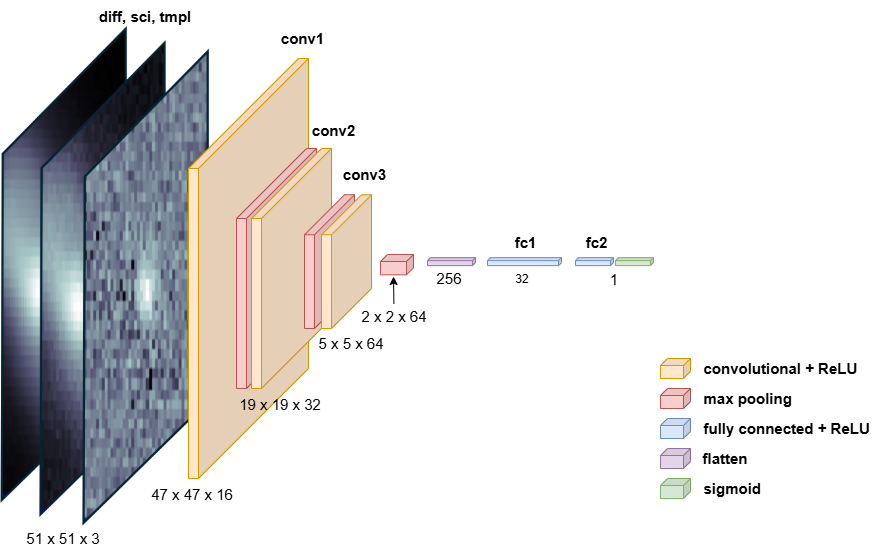
\includegraphics[width=0.8\linewidth]{figures/cnn_arch.png}
    \caption{CNN architecture of the Machine Learning model that generates a reliability score for every DIASource. The input data are the combined template, science, and the difference image postage stamps, each of size 51$\times$51 pixels, centered on the detected sources. The input array has a shape of (3, 51, 51). The CNN has three convolutional layers and two fully connected layers. The last layer has an output size of 1, and the sigmoid function is used for the output layer to provide a probabilistic interpretation. The design of the CNN is purposefully minimal to meet computational and time requirements.}
    \label{fig:cnn_arch}
\end{figure}
We developed a relatively simple model: a Convolutional Neural Network with three convolutional layers and two fully connected layers. The convolutional layers have a 5×5 kernel size, with 16, 32, and 64 filters, respectively. A max-pooling layer of size 2 is applied at the end of each convolutional layer, followed
by a dropout layer of 0.4 to reduce overfitting. The last
fully connected layers have sizes of 32 and 1. The ReLU
activation function is used for the convolutional layers
and the first fully connected layer, while a sigmoid function is used for the output layer to provide a probabilistic interpretation. The cutouts are generated by extracting postage stamps of 51$\times$51 pixels centered on the detected sources. The input data of the model consists of the template, science, and difference image stacked to have an array of shape (3, 51, 51) (See Figure \ref{fig:cnn_arch}). The model is implemented using PyTorch \citep{paszke2019pytorch}. The Binary Cross Entropy loss function is used, along with the Adaptive Moment Estimation (Adam) optimizer with a fixed learning rate of $1\times10^{-4}$, weight decay of $3.6\times10^{-2}$, and a batch size of 128. The design of the CNN is guided by the need to meet computational and timing requirements as specified in the `Data Management System Requirements' (DMSR, \cite{LSE-61}). While the model is architecturally conservative, we continuously test its performance against that of other models of demonstrated accuracy \citep[e.g.,][]{2026AJ....171..205I}, so as to direct our improvement towards either the model or the training data. At the time of writing, we identified that the most significant improvements can be achieved by improving the training data.



\section{Data}\label{sec:data}

The data to train the model has been in constant evolution, adjusting it every time to the most recent status of the telescope and data pipelines. For each model update, a specific dataset was used for training. Here, we described the three datasets used for \V1-\V3 models.

\subsection{Data for \V1 (DP1) model: LSSTComCam data}

The ML-Reliability model was initially trained with 89,066 \texttt{Real} and the same amount of \texttt{Bogus} labels, extracted from the Data Challenge 2 simulations \cite[DC2,][]{2021arXiv210104855L}, plus random injections of stars (i.e., PSFs at random locations without Galaxy associations) to increase the number of \texttt{Real}. Once the LSSTComCam data became available, the model was fine-tuned on a subset of that data containing 183,046 postage stamps with PSF injections. This fine-tuned model was the one used to generate reliability scores for Data Preview 1 \cite[DP1,][]{RTN-095} and is tagged \V1. 

\subsection{Data for \V2 and \V3 (DP2) model: LSSTCam and Zooniverse}

The model was retrained (fine-tuned) to improve performance on the commissioning LSSTCam data that will eventually be released as Data Preview 2 \cite[DP2][]{RTN-111}, leading to model version \V3. The \V2 model, as of April 2026, is being used for the AP pipeline and the production of alerts. The training of \V3, and \V2 relies partially and totally, respectively, on real data (no fake injection) and \texttt{Real}/\texttt{Bogus} labels obtained by the Zooniverse citizen scientists through the `Rubin Difference Detectives' project. The fine-tuned model will be used to generate reliability scores for DP2.
 
\subsubsection{Rubin Difference Detectives: Zooniverse Citizen Science Project}\label{sec:zooniverse}

Rubin Difference Detectives was launched on November 11th, 2025, with 242,391 DIA Sources (a ``subject'' in Zooniverse terms) for the Zooniverse citizen scientists to label. The distribution of the DIA sources per catalog is described in \autoref{tab:list_data}. By associating DIA detections in LSSTCam data with various catalogs (TNS \citep{tns_cite}, Gaia \citep{rimoldini2023gaia}, Rubin Solar System catalogs), and  DIA detections with \rel\ score between 0.5 and 0.9, \texttt{Real} labels generated by the \V1 model (subset tagged `reliability\_cuts')), and by using measured DIA source properties, we produced a dataset of DIA detections that is expected to be close to balanced in the \texttt{Real/Bogus} distribution.

\begin{table}
\footnotesize
    \centering
    \begin{tabular}{|c|c|c|c|c|c|}
    \hline
        \textbf{Name} & \textbf{handle}&\textbf{\# sources} & \textbf{Pipeline} & \textbf{Type}  \\ \hline
      
        tns\_ap & tns&219 & AP &TNS match\\\hline
        tns\_drp33 &tns&855 & DRP 2025\_33 &TNS match\\\hline
        tns\_drp37 &tns&984 & DRP 2025\_37 &TNS match\\\hline
        galaxy\_ddf & galaxy&10,932 & AP & Galaxy match (extendedness=1) \\ \hline
        rel\_cuts\_drp33\_gt\_05\_lt\_09 & reliability\_cuts&49,933 & DRP 2025\_33 &reliability cut\\\hline
        ss\_drp37 &ss&88,058 &DRP 2025\_37 & Solar System match \\ \hline
        gaia\_drp37 &gaia& 89,410 & DRP 2025\_37 &GAIA match\\\hline
           
    \end{tabular}
    \caption{Description of the DIA sources extracted from AP and DRP data by cross-matching with GAIA and TNS catalog, with the internal Solar System Catalogs, and with the sources with parameter \texttt{extendedness=1} given by Rubin source catalogs, and transients that received a $0.5<\rel<0.9$  score from the \V1 model. `Handle' refers to the short-hand label by which these sets will be referred to throughout the rest of this manuscript.}
    \label{tab:list_data}
\end{table}


The subjects given to the citizen scientists were images composed of three postage stamps of size 51$\times$51: template, science, and difference images, the DIA pixel output for each detected source. Volunteers were asked to perform the following task: \textit{Label the object seen in the center of the difference image as \texttt{Real} or \texttt{Bogus}}; no skip option was provided. \autoref{fig:zooniverse_screenshot} shows how the image, the task, and the answer options were presented to the volunteers. 

\begin{figure}[htbp]
    \centering
    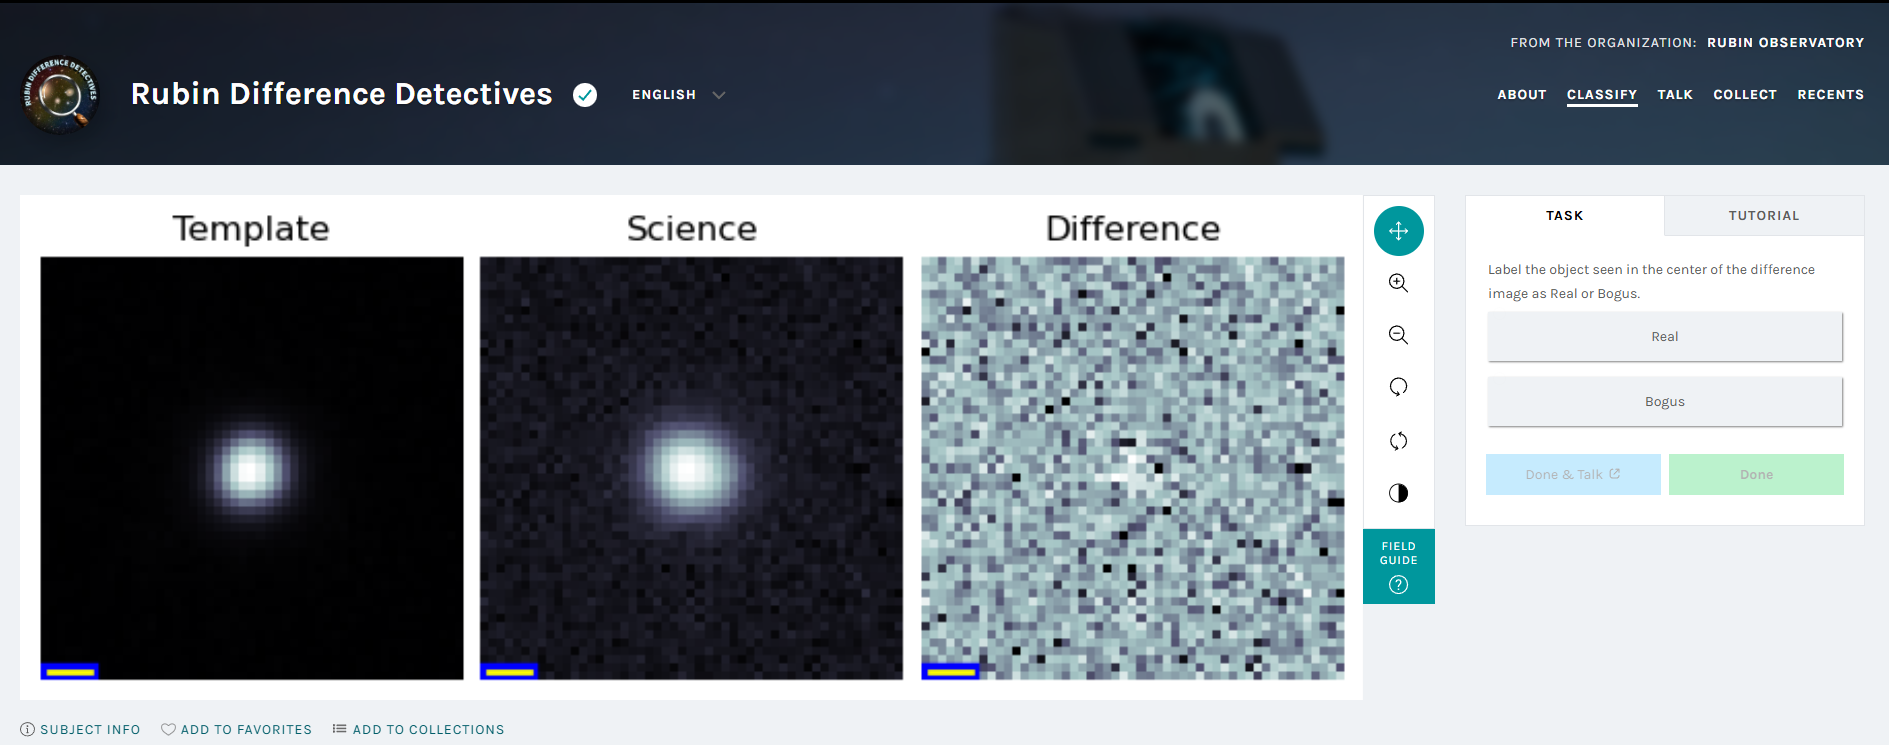
\includegraphics[width=1\linewidth]{figures/zooniverse_screenshot.png}
    \caption{Zooniverse interface of the Rubin Difference Detectives project. The citizen scientists were shown a subject, which is an image with the template, science, and the difference postage stamps, and they were asked to select whether the source in the difference image is \texttt{Real} or \texttt{Bogus}.}
    \label{fig:zooniverse_screenshot}
\end{figure}

For a subject to be ``retired'', meaning volunteers can no longer see it and labels are no longer collected, it first had to have been classified as either \texttt{Real} or \texttt{Bogus} by two different volunteers in agreement. If this initial condition was not met, the subject was instead retired after having been classified by seven different volunteers. 

The following section describes how the classifications given to a DIA source were used to determine the final \texttt{Real} or \texttt{Bogus} label, which, in the end, corresponded to the ground truth labels to train the reliability score model.




\subsubsection{Analysis of the Zooniverse classifications}\label{sec:bayesian}


The methodology we used to understand the classifications made by the volunteers and estimate the \texttt{Real}/\texttt{Bogus} classifier performance of the Rubin Difference Detectives project was a modification of the algorithm defined and implemented in \cite{marshall2016space}. %The labels obtained through this method are then the training/validation and testing labels to fine-tune the ML-reliability model. 
Following this work, we implemented a probabilistic classification for each subject ($\text{Pr}(\texttt{Real})$: probability of the DIA source to be a \texttt{Real} astrophysical object). %; the classifier was based on all the classifications given to the subject. 
Their probabilistic methodology relied on understanding how the volunteers responded to a reference data set (subjects where the ground truth was known) and thus building a prior for each user. The probabilistic classifier is explained in great detail in \cite{marshall2016space}. We refer the reader to their paper. 
Our reference data set was composed of either the DIA sources classified by the Oxford team (8 experts from the University of Oxford who classified a fraction of the DIA sources in Zooniverse (Weston et al. in preparation)), the DIA sources classified by the Rubin-ML-Reliability team (referred to as Rubin hereafter), or both. The reference set had a total of 20,261 (\texttt{Real}: 8576, \texttt{Bogus}: 11,686) DIA sources, when considering both reference datasets, and a total of 8956 (\texttt{Real}: 3805, \texttt{Bogus}: 5151)  DIA sources, when considering only the Rubin expert labels.  We note here that we only consider volunteers who provided labels for at least one subject in the reference set. At the time of training model version \V2, out of 3750 volunteers, only 2476 encountered a DIA source of the Rubin reference data set (2792 when considering both reference datasets). 

Because the number of labels is typically much smaller in `Rubin Difference Detectives' compared to the `Space Warp' project that inspired \cite{marshall2016space}, we implement the following modifications: 
\begin{itemize}
\item{We set a minimum threshold of 0.05 and a maximum threshold of 0.95 to the participants' Bayesian prior to avoid collapse of the posterior (e.g., if a volunteer only labeled one reference source, their prior would be 0 or 1, depending, causing the posterior to collapse to the same value);}
\item{We implement a stability criterion to accept a subject's label as described below.}
\end{itemize}

Since the $\text{Pr}(\texttt{Real})$ per DIA source returned a float between 0 and 1, to determine the final binary classification (\texttt{Real} = 1 or \texttt{Bogus} = 0), we defined two different scenarios. 
\begin{enumerate}
    \item \textit{stable set}: A source is considered stable if (1) the probability of being \texttt{Real}, $\text{Pr}(\texttt{Real})$, meets a threshold ($\geq 0.90$ for \texttt{Real}, $\leq 0.10$ for \texttt{Bogus}) and (2) this condition holds for at least the last three classifications.
    \item \textit{unstable set}: Only the threshold condition applies, without the stability criterion.
\end{enumerate}

\begin{figure}[htb!]
    \centering
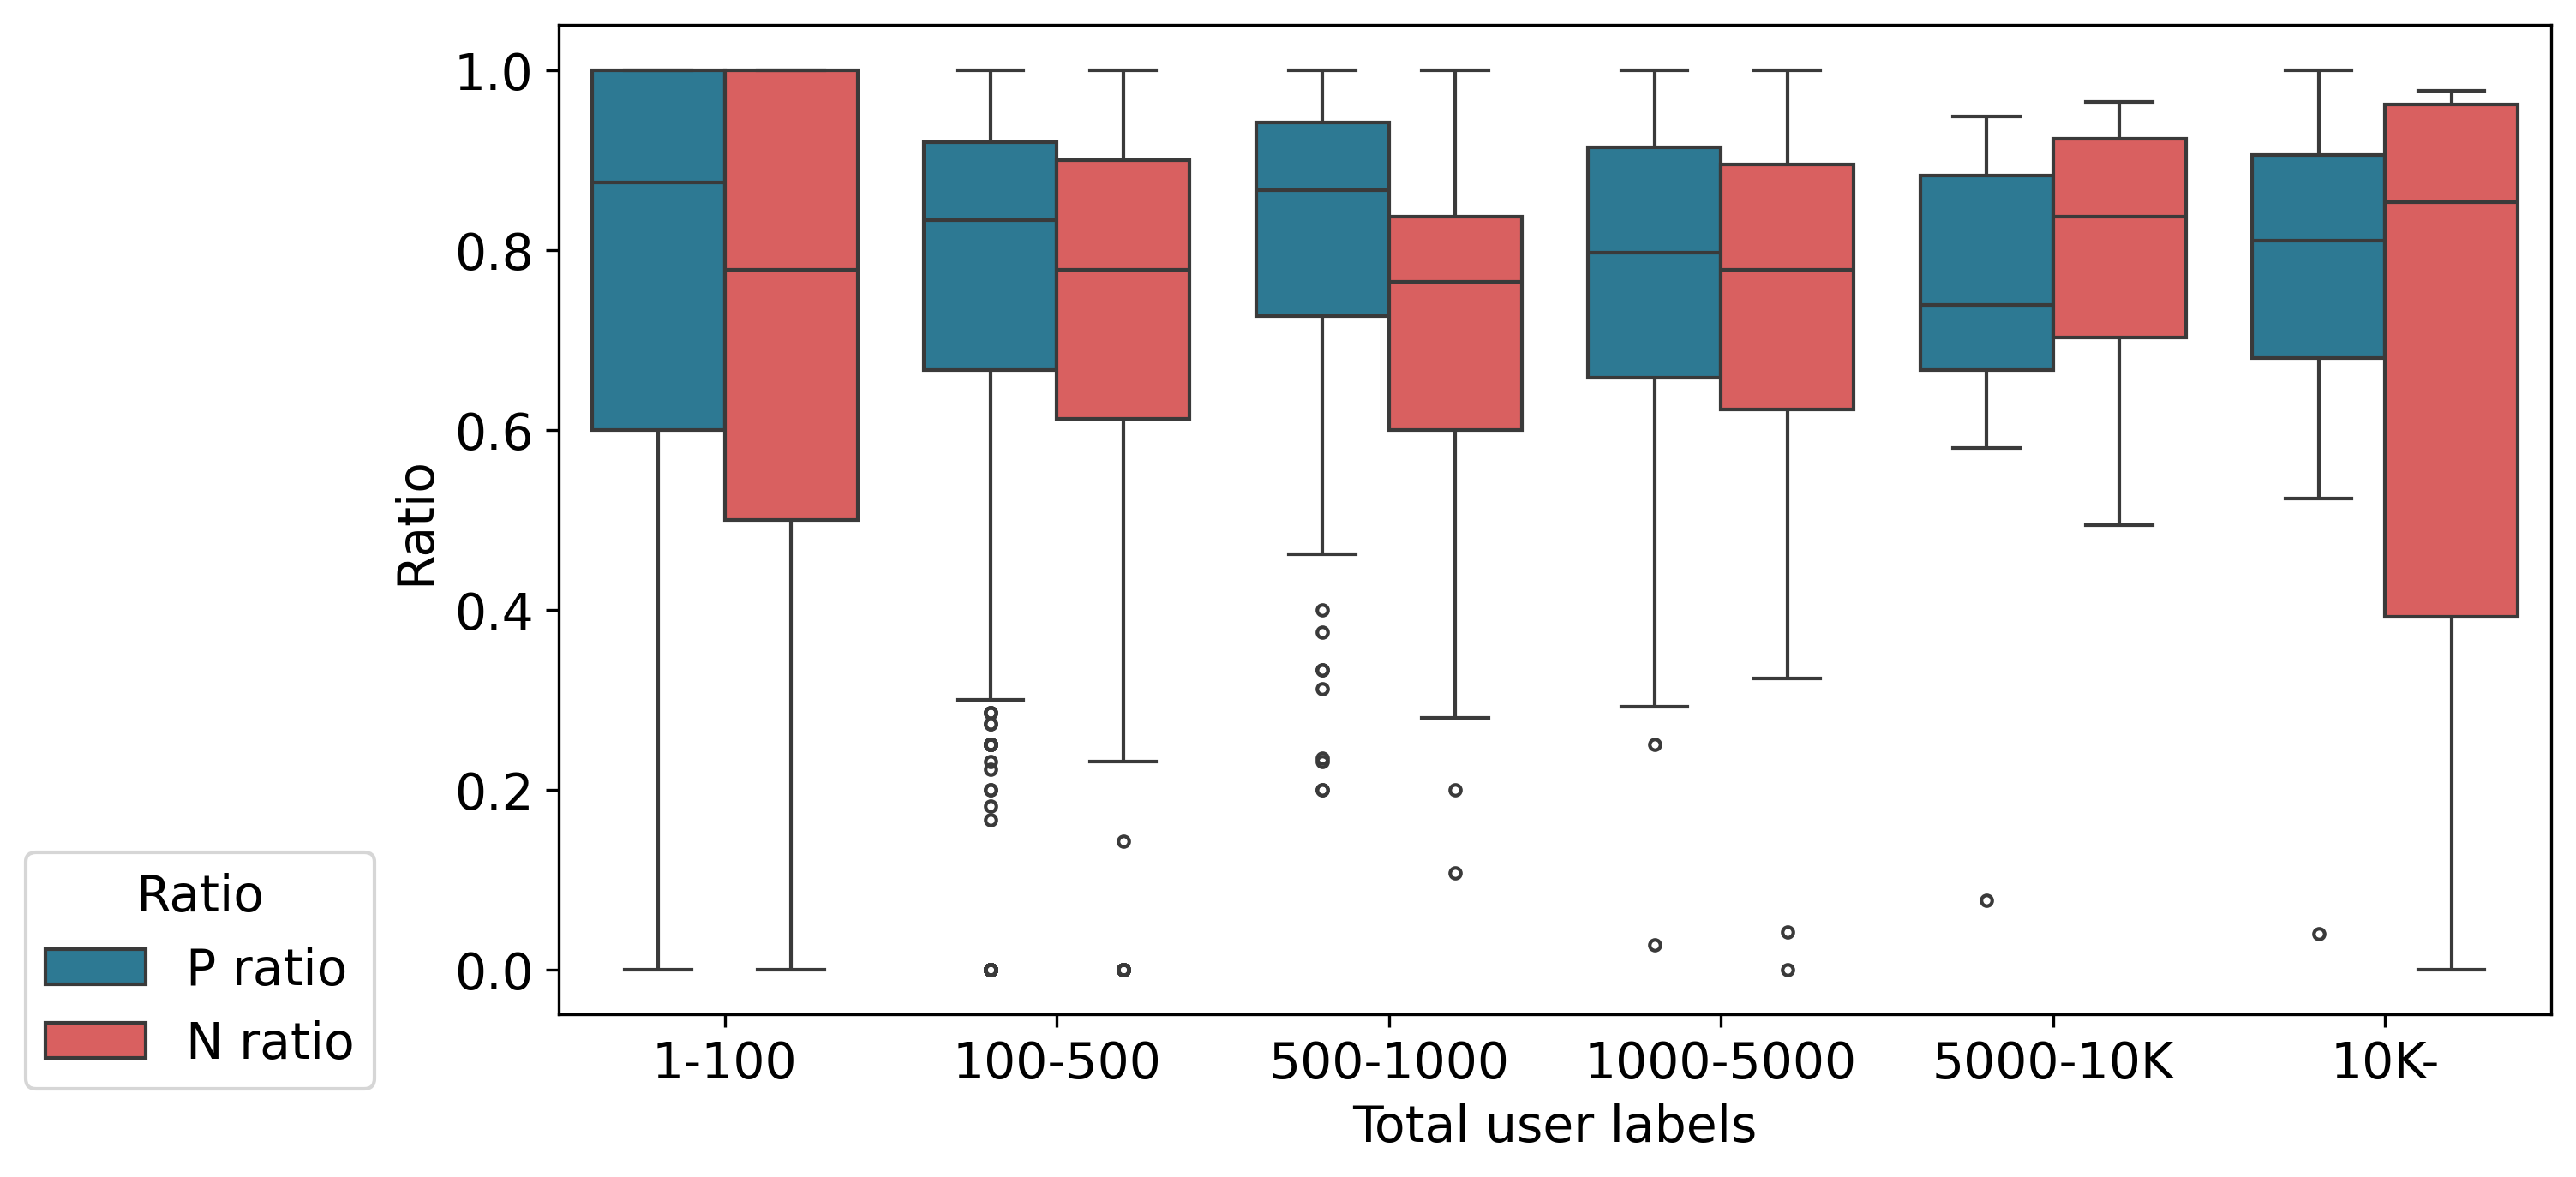
\includegraphics[width=0.8\linewidth]{figures/tns_tps_ratio_users.png}
    \caption{Fraction of Positives (P) and Negatives (N) labels obtained by comparing Zooniverse volunteer classification and reference classification (perfect agreement with the reference label would lead to a ratio of 1), per total classifications made by the user. %\tocheck{In general, the more classifications, the better the P and N ratio.} 
    The larger distributions for the 1-100 and >10k user labels is due to small number statistics.
    There are some outliers where the volunteers are very optimistic and classify everything as \texttt{Real}, or very pessimistic and classify everything as \texttt{Bogus}. Those users could be discarded, but in the Bayesian framework described in \cite{marshall2016space}, the impact of their labels is naturally suppressed.}
    \label{fig:tptn_ratio_users}
\end{figure}

In \autoref{fig:tptn_ratio_users}, we showed the fraction of Positives (P) and Negatives (N) labels ($ N_\text{P}/N_\text{P labels}$ and $N_\text{N}/N_\text{N labels}$ respectively) obtained by comparing volunteer classification and reference data labels as a function of the number of labels provided by the volunteer. In general, the more subjects a volunteer labels, the higher the P and N fractions. Ideally, the P and N fractions should be similar, indicating that the user can distinguish \texttt{Real} and \texttt{Bogus} sources and is not biased toward one class.



The distribution of \texttt{Real}/\texttt{Bogus} for the reference data changes depending on the type of source (\texttt{gaia}, \texttt{galaxy}, \texttt{reliability\_cuts}, \texttt{ss}, or \texttt{tns}, see \autoref{tab:list_data}), and it is also related to the Signal to Noise Ratio (SNR) of the DIA source. Visual inspection of some DIA sources labeled by experts (
\autoref{fig:gt_snr_byset}) showed that low SNR tends to be classified as \texttt{Bogus}, regardless of the type of source.

\begin{figure}[htb!]
    \centering
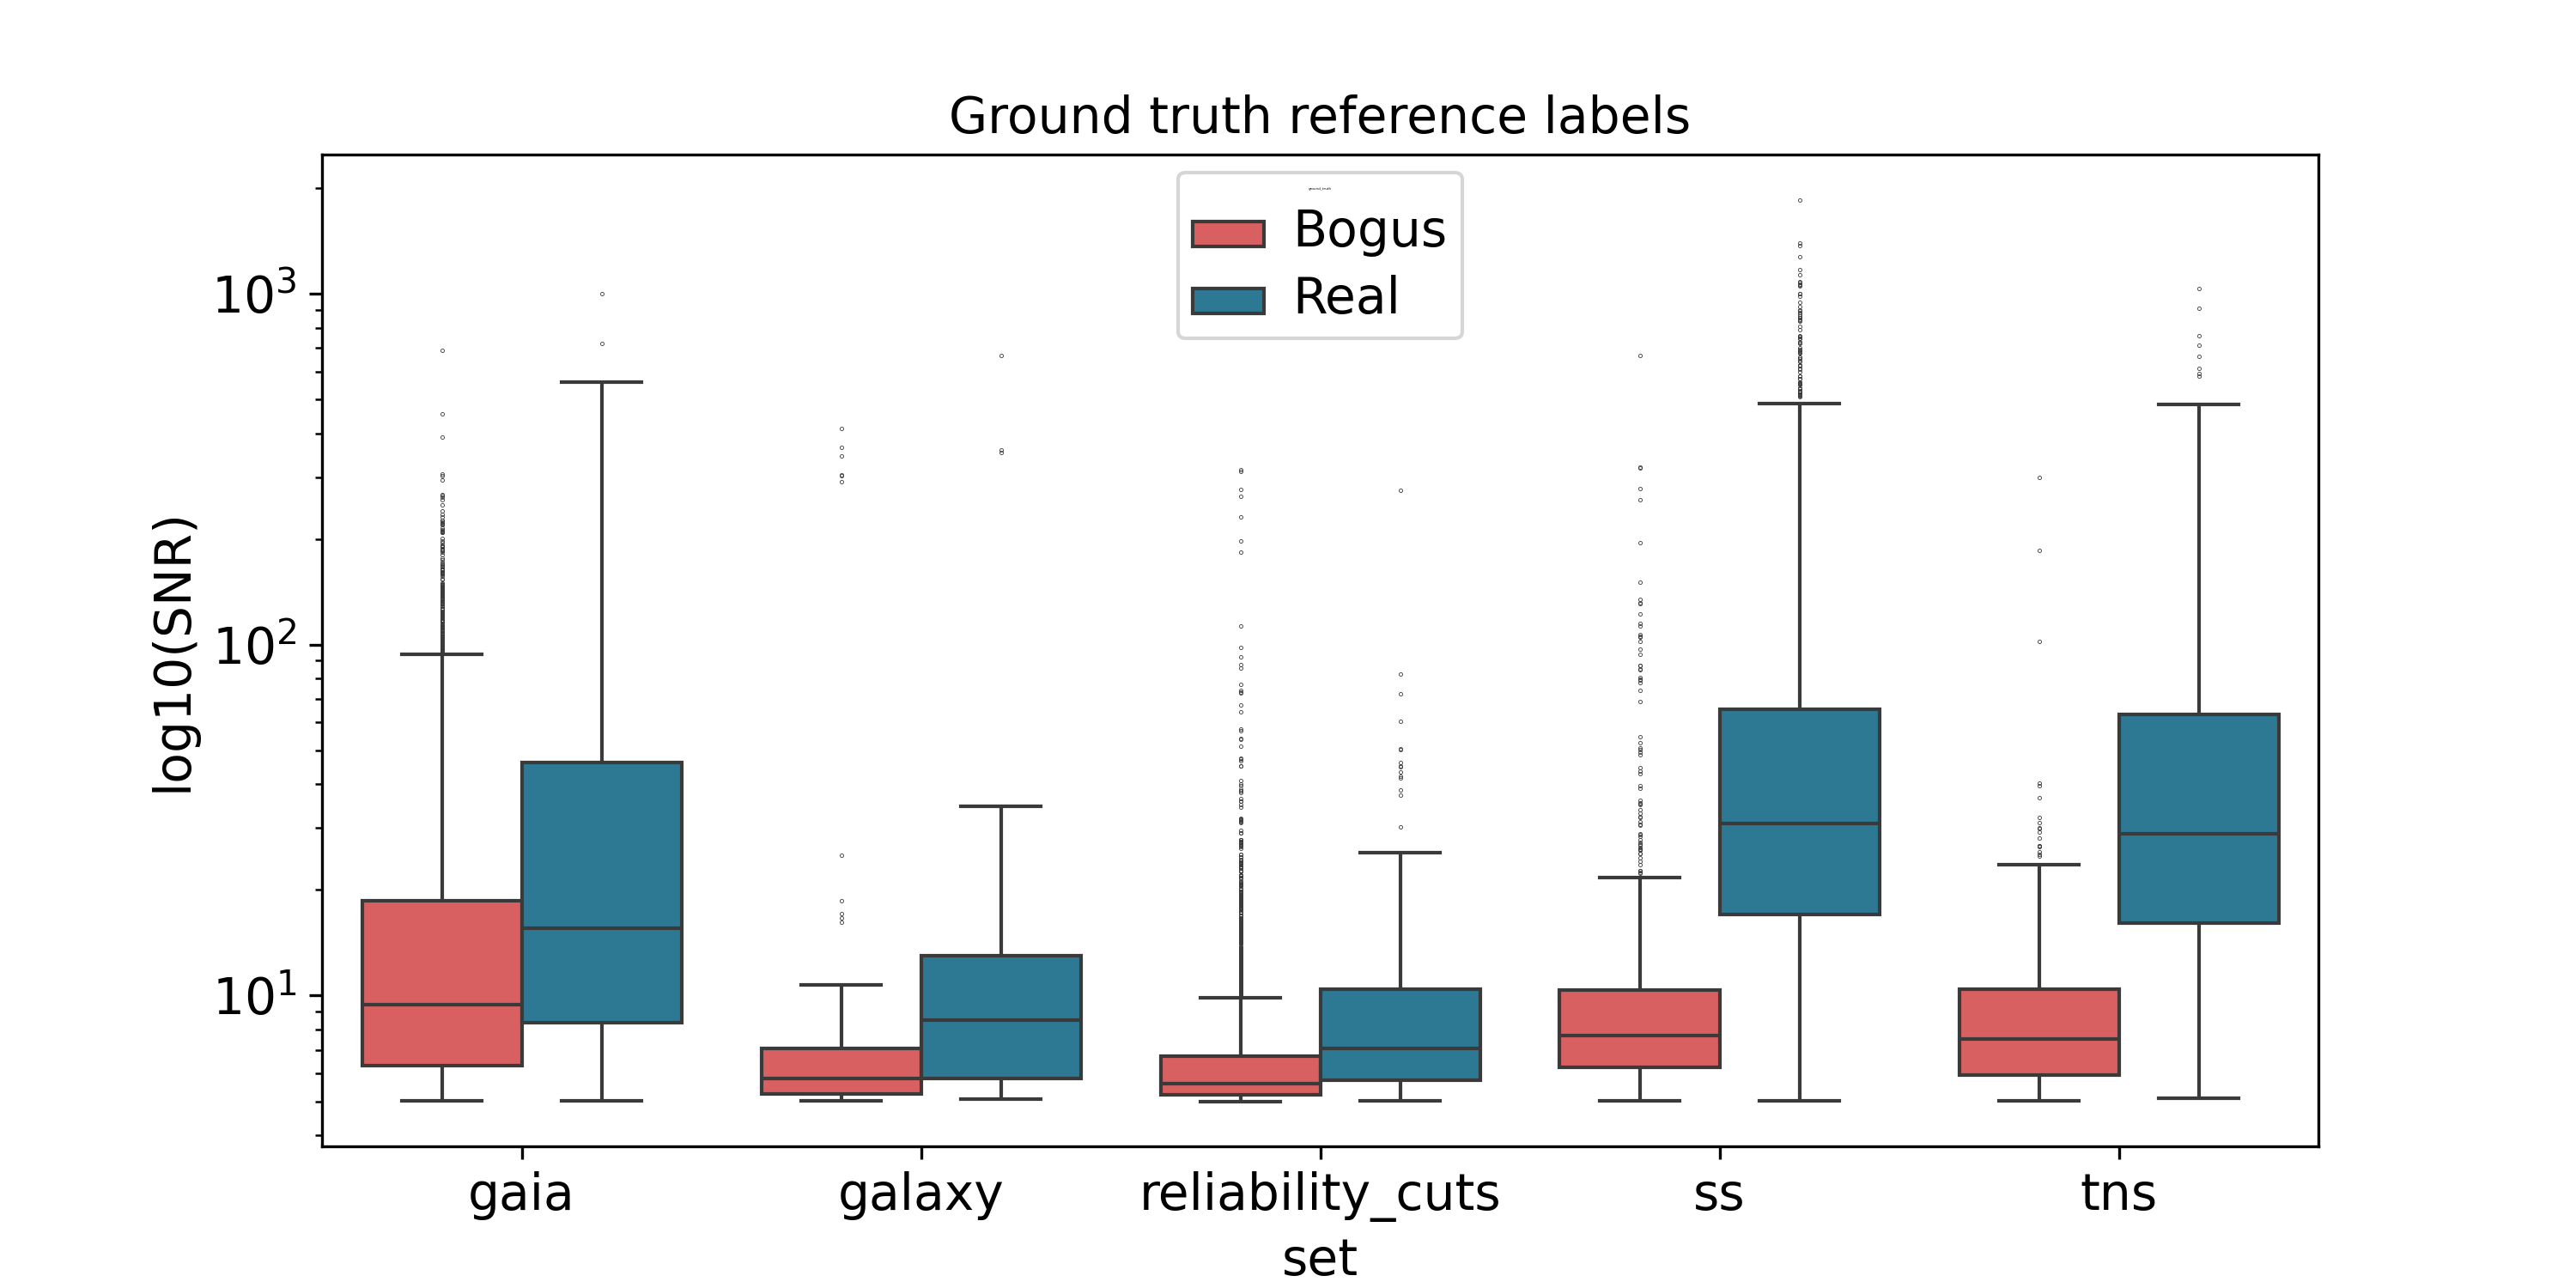
\includegraphics[width=0.8\linewidth]{figures/gt_labels_snr_byset.png}
    \caption{Signal to Noise Ratio (SNR) distribution for each source in the respective catalogs for DIA sources labeled by experts as \texttt{Real} (blue) or \texttt{Bogus} (red).}
    \label{fig:gt_snr_byset}
\end{figure}

% Using these volunteer classifications, we constructed balanced datasets (same amount of \texttt{Real} and \texttt{Bogus}) for model training.

% \subsection{Final Data Description}
After applying the Bayesian approach (\citealt{marshall2016space}) to the Zooniverse classification, the breakdown of labels is described in \autoref{tab:total_data_zoo_analysis}.
\begin{table}[htb!]
    \centering
    \begin{tabular}{|c|c|c|c|}
    \hline
       \textbf{Scenario}  & \textbf{Total \texttt{Real}} & \textbf{Total \texttt{Bogus}} & \textbf{Reference Data} \\ \hline
       
        stable & 8236 & 40,402& Rubin\\ \hline
        unstable & 25,218& 53,024& Rubin\\ \hline
        \hline \hline
        stable & 8025 & 46,124 & Oxford and Rubin\\ \hline
        unstable & 23,889& 57,570& Oxford and Rubin\\ \hline
    \end{tabular}
    \caption{Final count of \texttt{Real} and \texttt{Bogus} obtained after determining the probability of the source being \texttt{Real} given the classifications provided by the Zooniverse volunteers following the criteria described in \autoref{sec:bayesian}.}
    \label{tab:total_data_zoo_analysis}
\end{table}

The total number of \texttt{Real} and \texttt{Bogus} labels after the classification analysis is highly unbalanced; for the purpose of training a binary classification machine learning model, the data sets should be balanced between classes to avoid inducing a bias. The model performance results shared hereafter are based on a balanced data set, produced by subsampling the data shown in \autoref{tab:total_data_zoo_analysis}. The distribution of the \texttt{Real} and \texttt{Bogus} by data origin, as explained in \autoref{tab:total_data_zoo_analysis}, after analyzing the Zooniverse classifications, is shown in \autoref{fig:posterior_byset}.

\begin{figure}[htb!]
   \centering
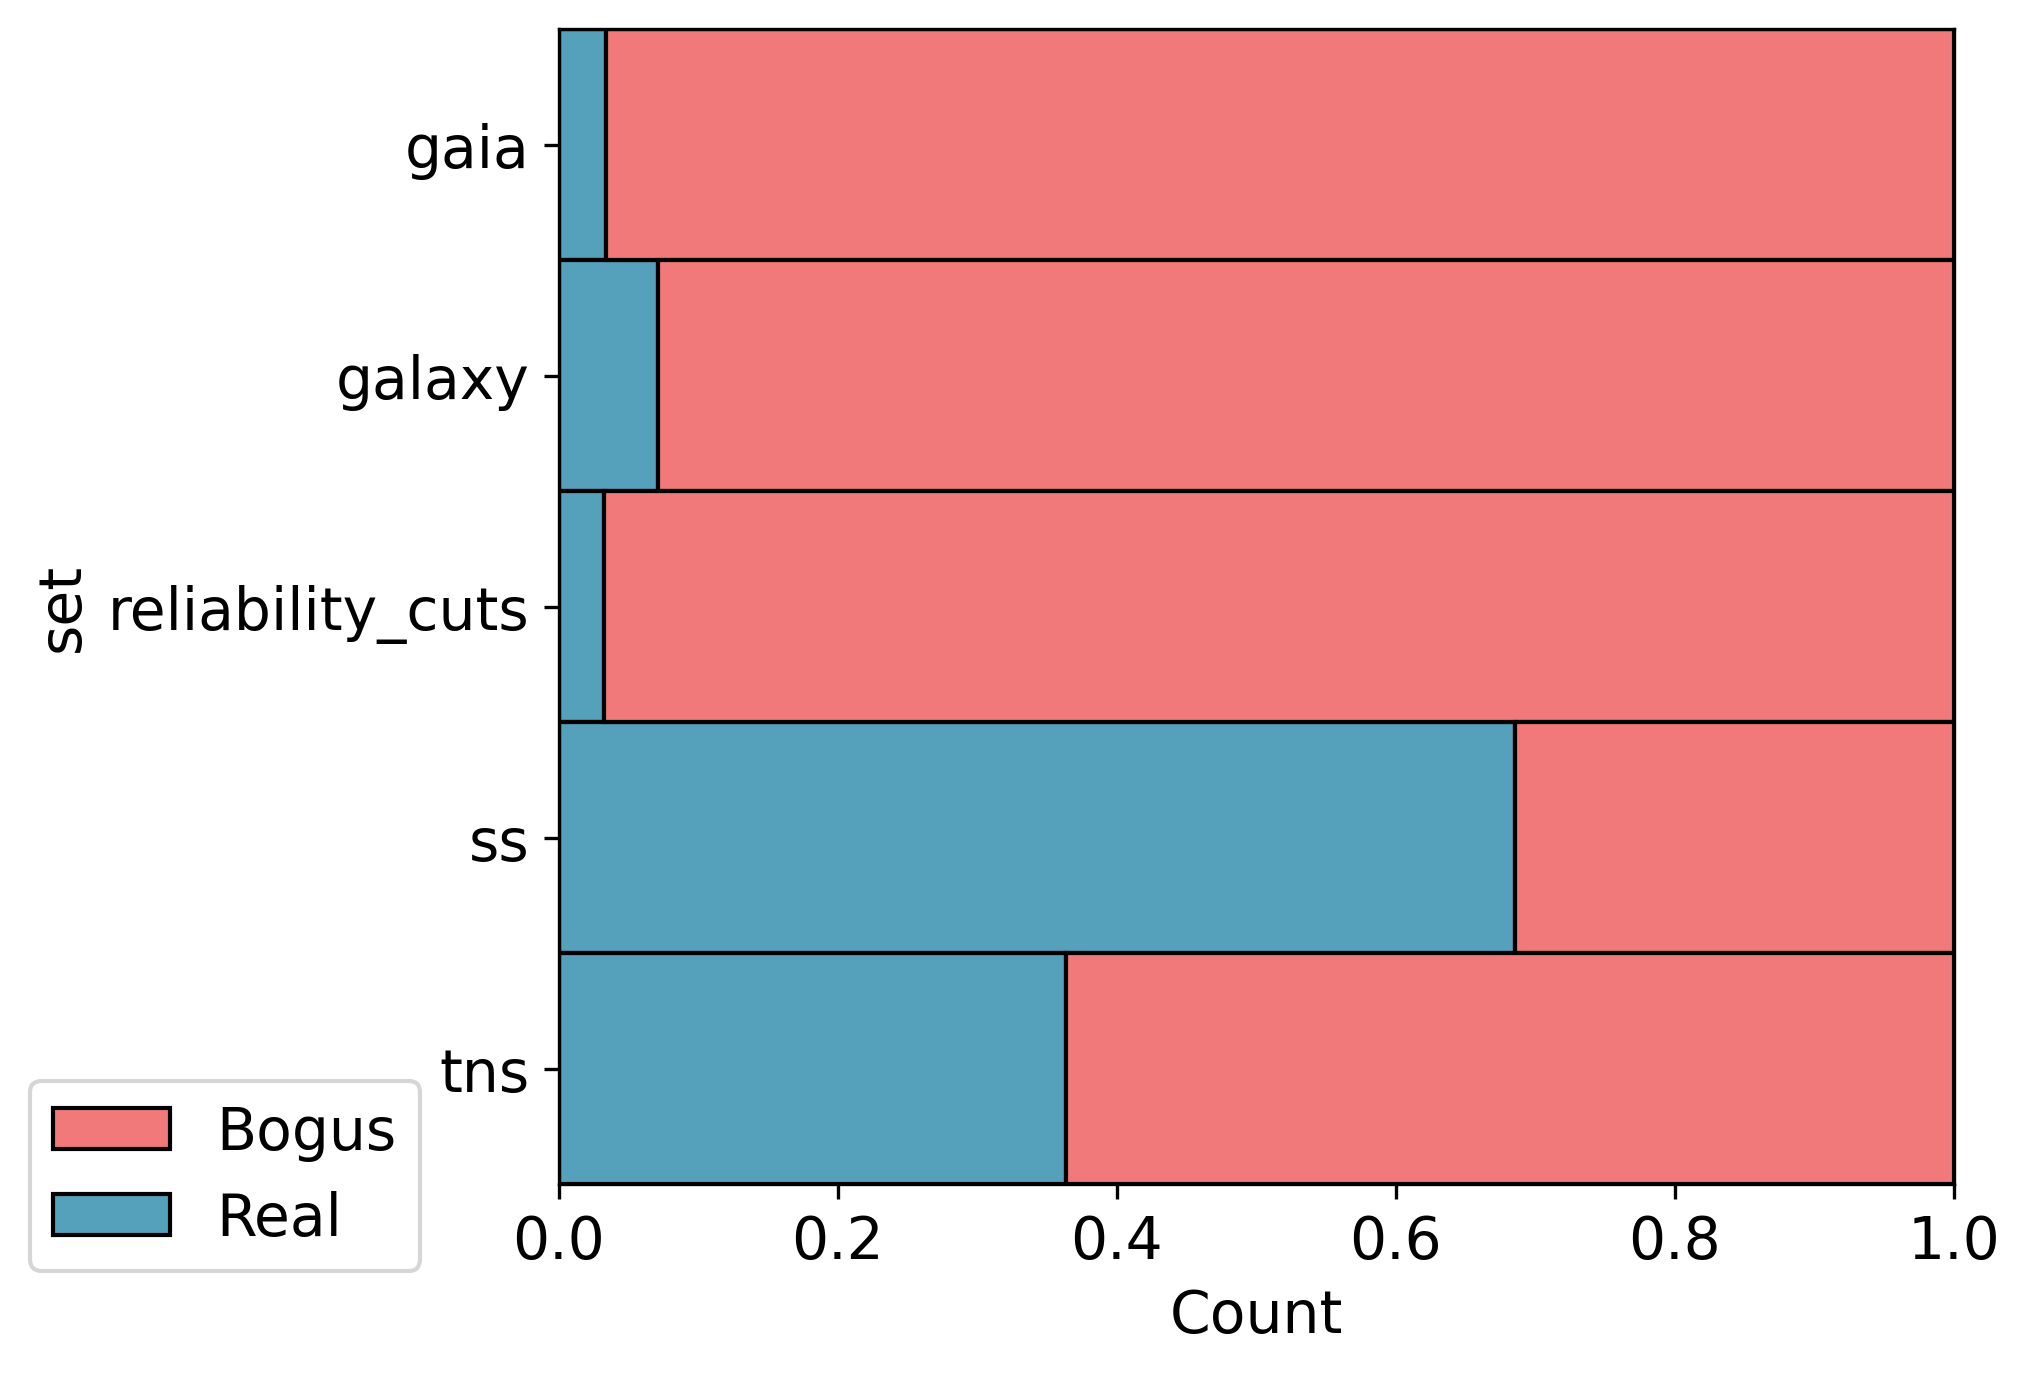
\includegraphics[width=0.6\linewidth]{figures/posterior_byset.png}
    \caption{Distribution of \texttt{Real} and \texttt{Bogus} as labeled via the `Rubin Difference Detectives' Zooniverse project for data used for training/validation/testing of the ML-reliability model \V2 and \V3. The data is grouped as in \autoref{tab:list_data}. %: tns\_ap, tns\_drp33, and tns\_drp37 are all presented under `tns', and the same for data obtained after cross-matching with the GAIA catalog.  
    %Distribution of each data origin for each class, \texttt{Real} (1) and \texttt{Bogus} (0). 
    Almost 80\% of the \texttt{Real} labels correspond to Solar System objects (`ss'), 10\% correspond to variable objects matched with the GAIA catalog, and the other 10\% is distributed between transients (TNS catalog), objects with extendendness = 1 (`galaxy'), and \texttt{Real} found by the \V1 model (`reliability\_cuts'). On the other hand, almost 60\% of the \texttt{Bogus} objects correspond to matches with the GAIA catalog, which we find are mainly due to bad subtractions, 25\% correspond to DP1 false positives (`reliability\_cuts'), and the remaining 15\% correspond to artifacts in the Solar System objects (`ss'), objects with extendendness = 1 (`galaxy'), and a few artifacts from matches with the TNS catalog. }
\label{fig:posterior_byset}
\end{figure}

The construction of the ground truth labels for fine-tuning the \V2 and \V3 models relied on the Zooniverse analysis obtained by only considering the Rubin reference data set (see \autoref{tab:total_data_zoo_analysis}). Additionally, only detections with high-confidence labels (stable) were used. In total, 13,178 sources were used to fine-tune the \V2 and \V3 models: 6,630 \texttt{Real} and 6,548 \texttt{Bogus}. 1,647 were used to validate, and another 1,647 to test the model. Given the small size of the training data set, in addition to the original images, two augmentations (vertical and horizontal flipping) were added to the training. For \V3, a fraction of the dataset used for the \V1 DP1 model (LSSTComCam fakes) was also used. For \V2 the fine-tuning relies 100\% on the Zooniverse data.




\subsection{Data for Future models}
Future model iterations will include ground truth labels for fine-tuning the model, relying on the Zooniverse analysis obtained by considering the training data set of both the Oxford team and the Rubin-ML-Reliability team (see \autoref{tab:total_data_zoo_analysis}). Additionally, fake sources injected in more recent injection runs can be included. 






\section{Performance}

The distribution of the \rel\ score for a random set of DIA sources is shown in \autoref{fig:distribution_rel_score_versions} for all three model versions. Besides the peaks at $0$ and $1$, each model presents a third peak at $\sim 0.5$ for \V1 model, and $\sim 0.3$ for both the \V3 and \V2 models. The peak corresponds to when the science and difference images contain some rows or columns full of \texttt{NaN} values. 

\begin{figure}[htb!]
    \centering
    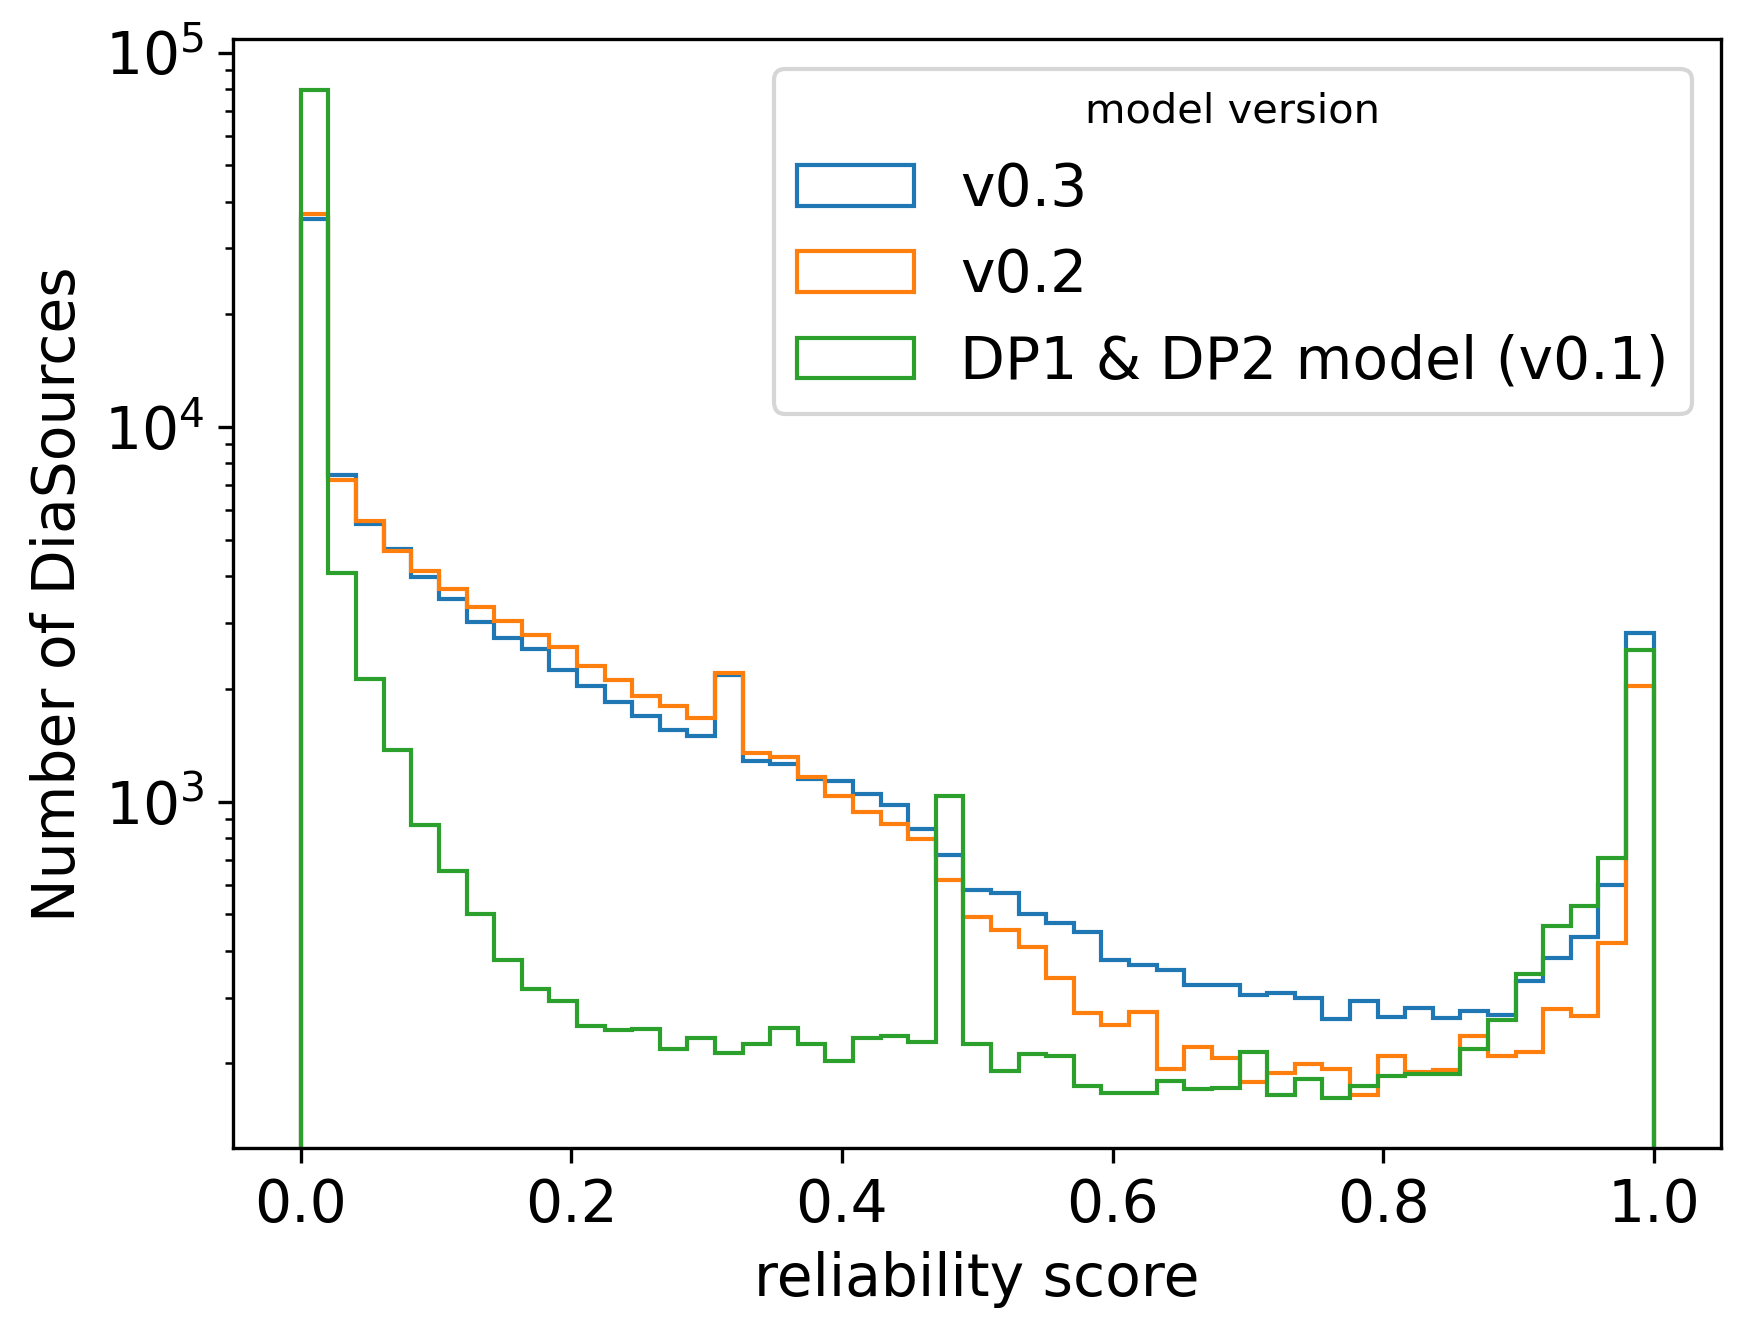
\includegraphics[width=0.6\linewidth]{figures/dist_rel_version.png}
    \caption{Distribution of the reliability score for each model version.}
    \label{fig:distribution_rel_score_versions}
\end{figure}

Given the high volume of DIA sources produced by the AP at the moment of writing, and to mitigate the impact on APDB, when generating alerts and identifying detections for downstream analysis (e.g., forced photometry), a reliability value cutoff is implemented for each model. The cutoff is determined by analyzing the behavior of the model against properties of the DIA sources, and the behavior on fakes, e.g. \autoref{fig:cosmos_compare_models}, \autoref{fig:st_apflux}, \autoref{fig:st_apflux_cutoff}, and \autoref{fig:psf/psferr_rel}. This cutoff also reduces the amount of \texttt{Bogus} that reaches the Brokers and the scientific community. The current cutoff values are 0.1, 0.5, and 0.5 for \V1 model, \V2, and \V3 model, respectively. We expect to lower that threshold for future versions of the ML-Reliability model.


The behavior of each model against SNR for a fake injection run outside of the training data set (see \autoref{sec:v01}) is shown in \autoref{fig:cosmos_compare_models}. As a reminder to the reader, the \V1 model was trained only using fakes; \V2 was only trained with real data without fake injection, and the \V3 model was trained with both fakes and real data. The slope of the distribution of \rel\ for \V2 as a function of SNR in the region $0\leq\text{SNR}\lesssim12$ indicates a model bias which we attribute to a bias in the volunteer's label, as discussed in \autoref{sec:bayesian} (see \autoref{fig:gt_snr_byset}). This bias is mitigated by the inclusion of fakes (injections) in the \V3 model data.

\begin{figure}[htb!]
    \centering
    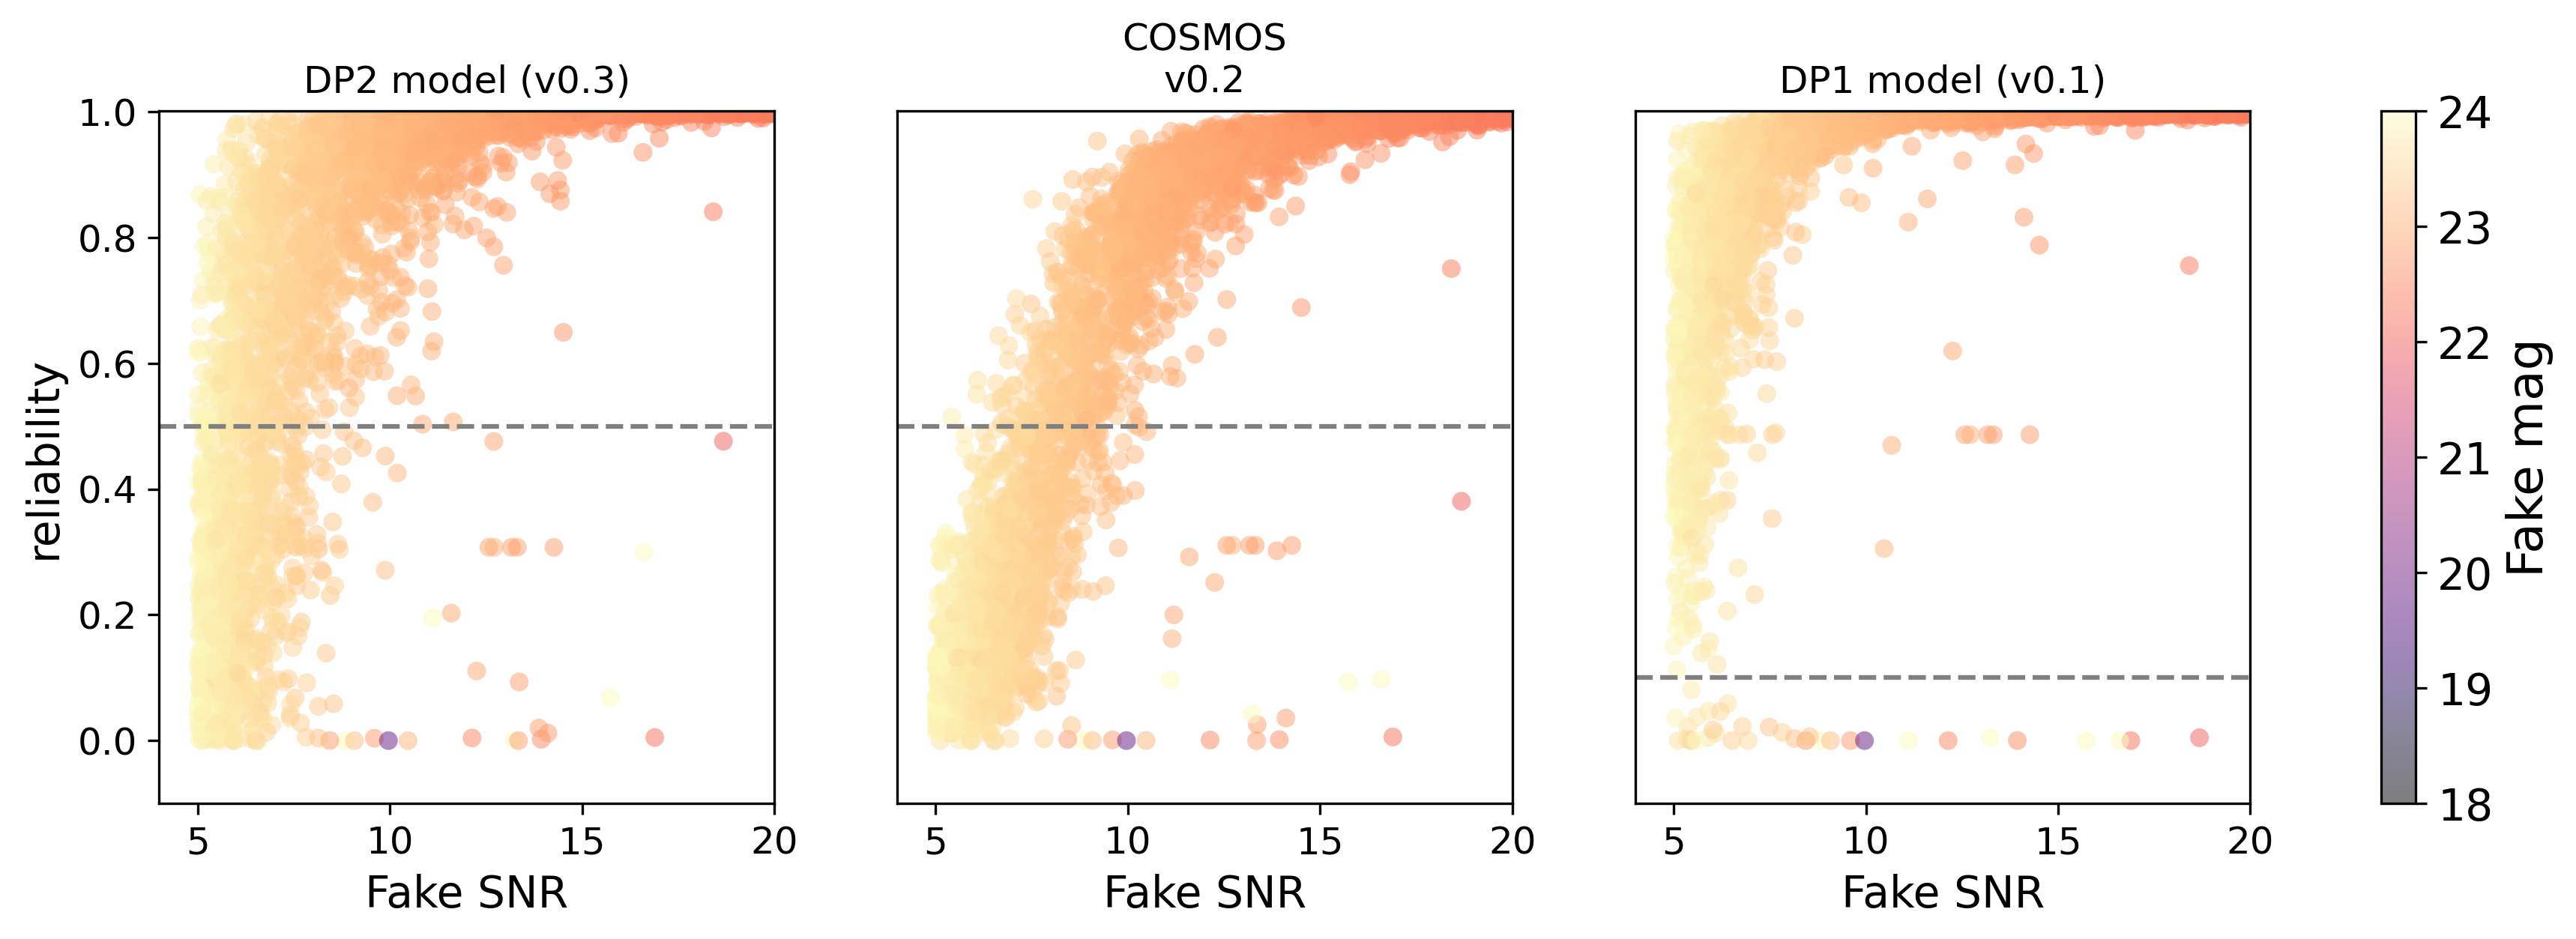
\includegraphics[width=1\linewidth]{figures/cosmos_compare_models.png}
    \caption{Reliability score against SNR for each model version for a set of fakes DIA sources in the magnitude range $m=24-21$ from an injection run outside of the training set. The horizontal dashed line indicates the \rel\ cutoff for each model version: 0.1 for \V1 and 0.5 for both \V2 and \V3.%\tocheck{We note a single extremely bright injection ($mag\sim20$ is assigned $\rel=0$. }
    }
    \label{fig:cosmos_compare_models}
\end{figure}


Following the basic idea behind the DIA, where the flux of the DIA source $F_{\text{Diff}}$ in the difference image is expected to be the subtraction of the science flux from the template flux, we show the flux measured by aperture photometry on the difference image $F_{\text{AP}}$ against the flux measured in the science and template images $F_{\text{Diff}}$ in \autoref{fig:st_apflux}. In an ideal case, these two values should follow a 1-1 relation (linear relation), and we would expect to have high reliability scores for DIA sources that fall on or near the diagonal in \autoref{fig:st_apflux}. Deviation from that diagonal may indicate some deviation from the basic flux measurement, and therefore a potential \texttt{Bogus} object, which should produce a low reliability score. \autoref{fig:st_apflux_cutoff} shows the same data but with the current reliability cutoffs applied ($\rel=0.1$ for \V1, $\rel=0.5$ for \V2 and \V3). Generally, we see a strong and encouraging dependence of \rel\ with the ratio of DIA and science-template flux, with deviation mostly near ($F_{\text{AP}},F_{\text{Diff}}) = $(0,0), where low SNR sources tend to get low \rel\ scores, as seen before. We also see an excess of $\rel>0.5$ for \V2 and \V3 throughout the lower left quadrant of the plot ($F_{\text{AP}}<0$ and $F_{\text{Diff}}<0)$, i.e. negative flux sources), while these sources receive extremely low scores in \V1 because this model was not trained on negative flux detections. We note that negative sources are likely to be uncharacteristically common in the current DP1 and DP2 DIA due to the proximity in time of the template generation with the science image collection, and to the short timeline during which the templates were constructed.

\begin{figure}[htb!]
    \centering
    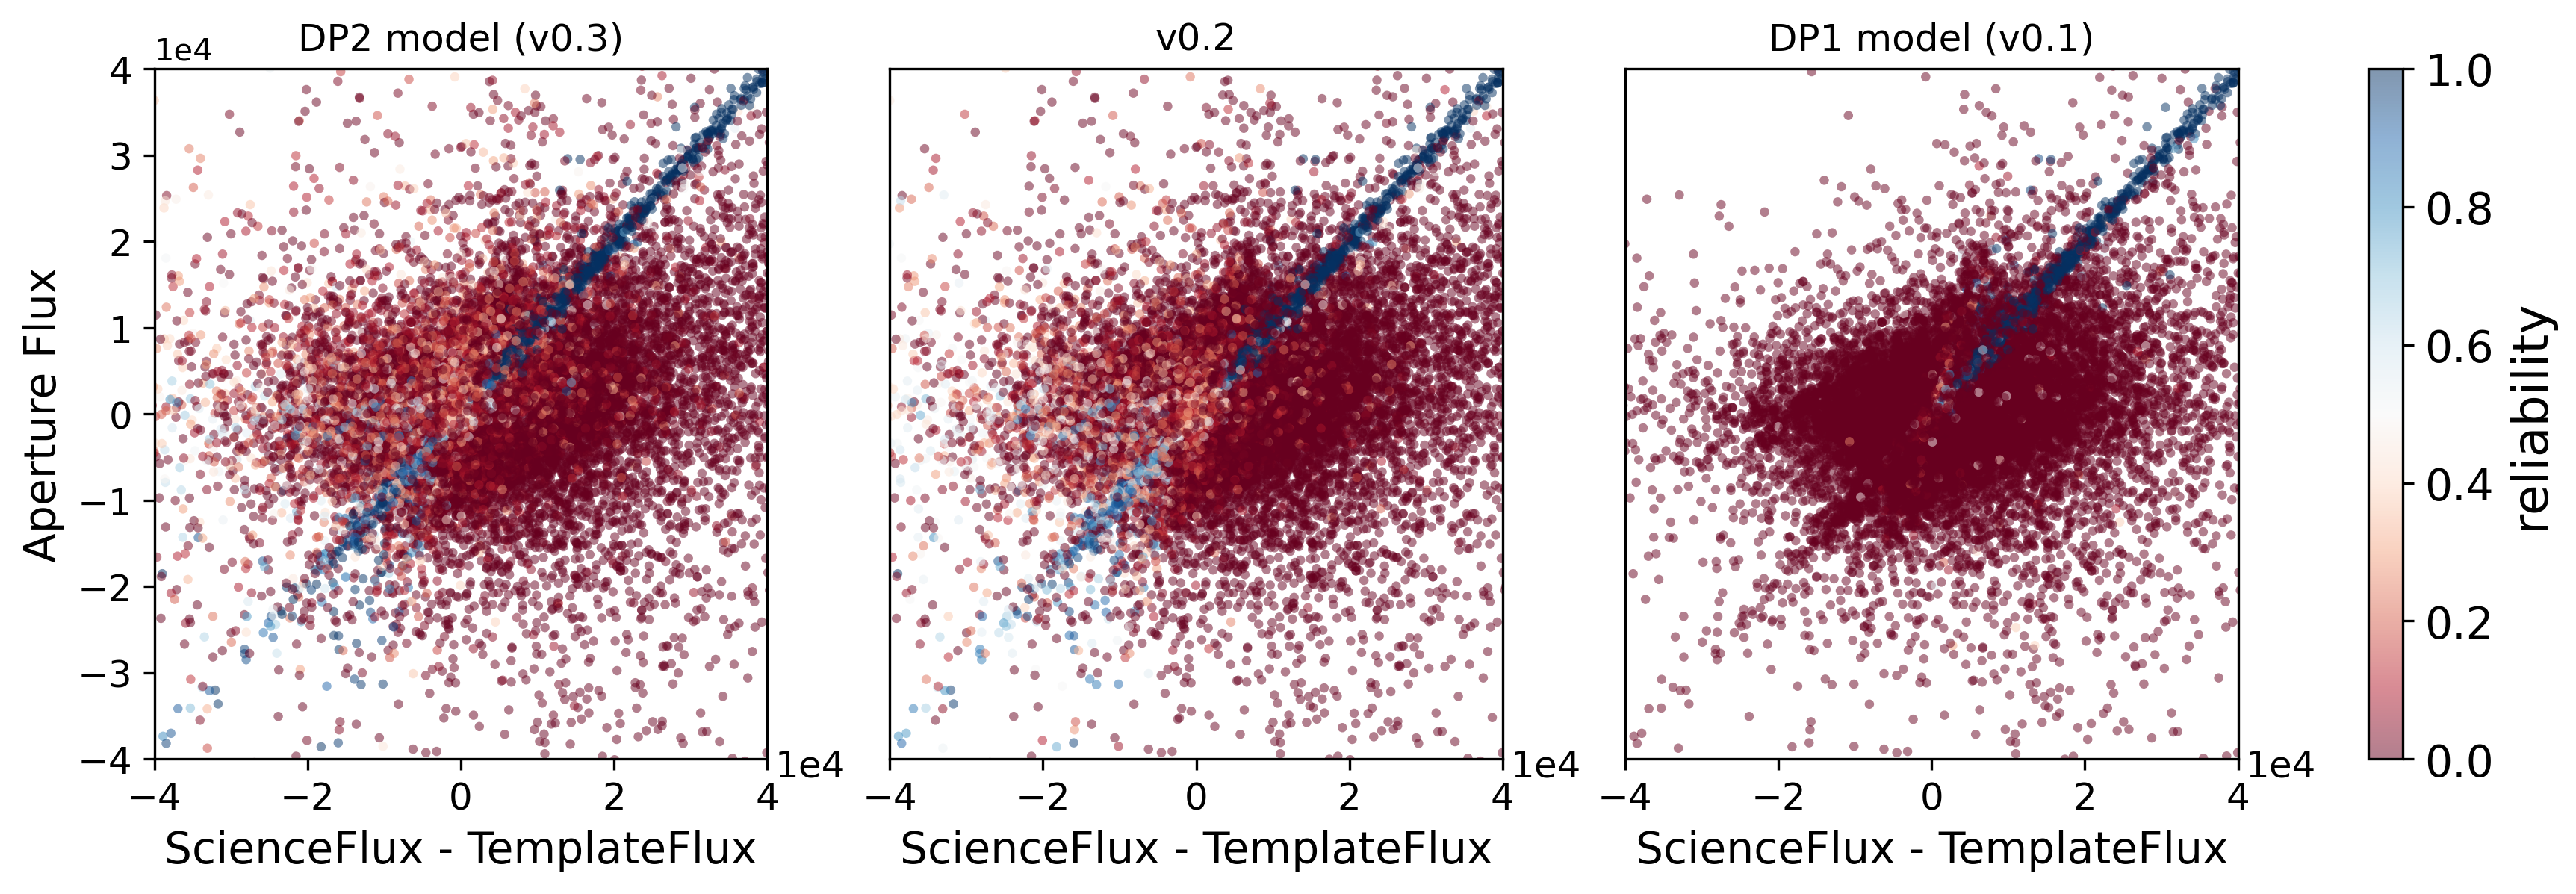
\includegraphics[width=1\linewidth]{figures/apfluxl_version.png}
    \caption{DIA Aperture Flux vs ScienceFlux - TemplateFlux colored by the reliability score for each model version for a random set of DIA sources.}
    \label{fig:st_apflux}
\end{figure}

\begin{figure}[htb!]
    \centering
    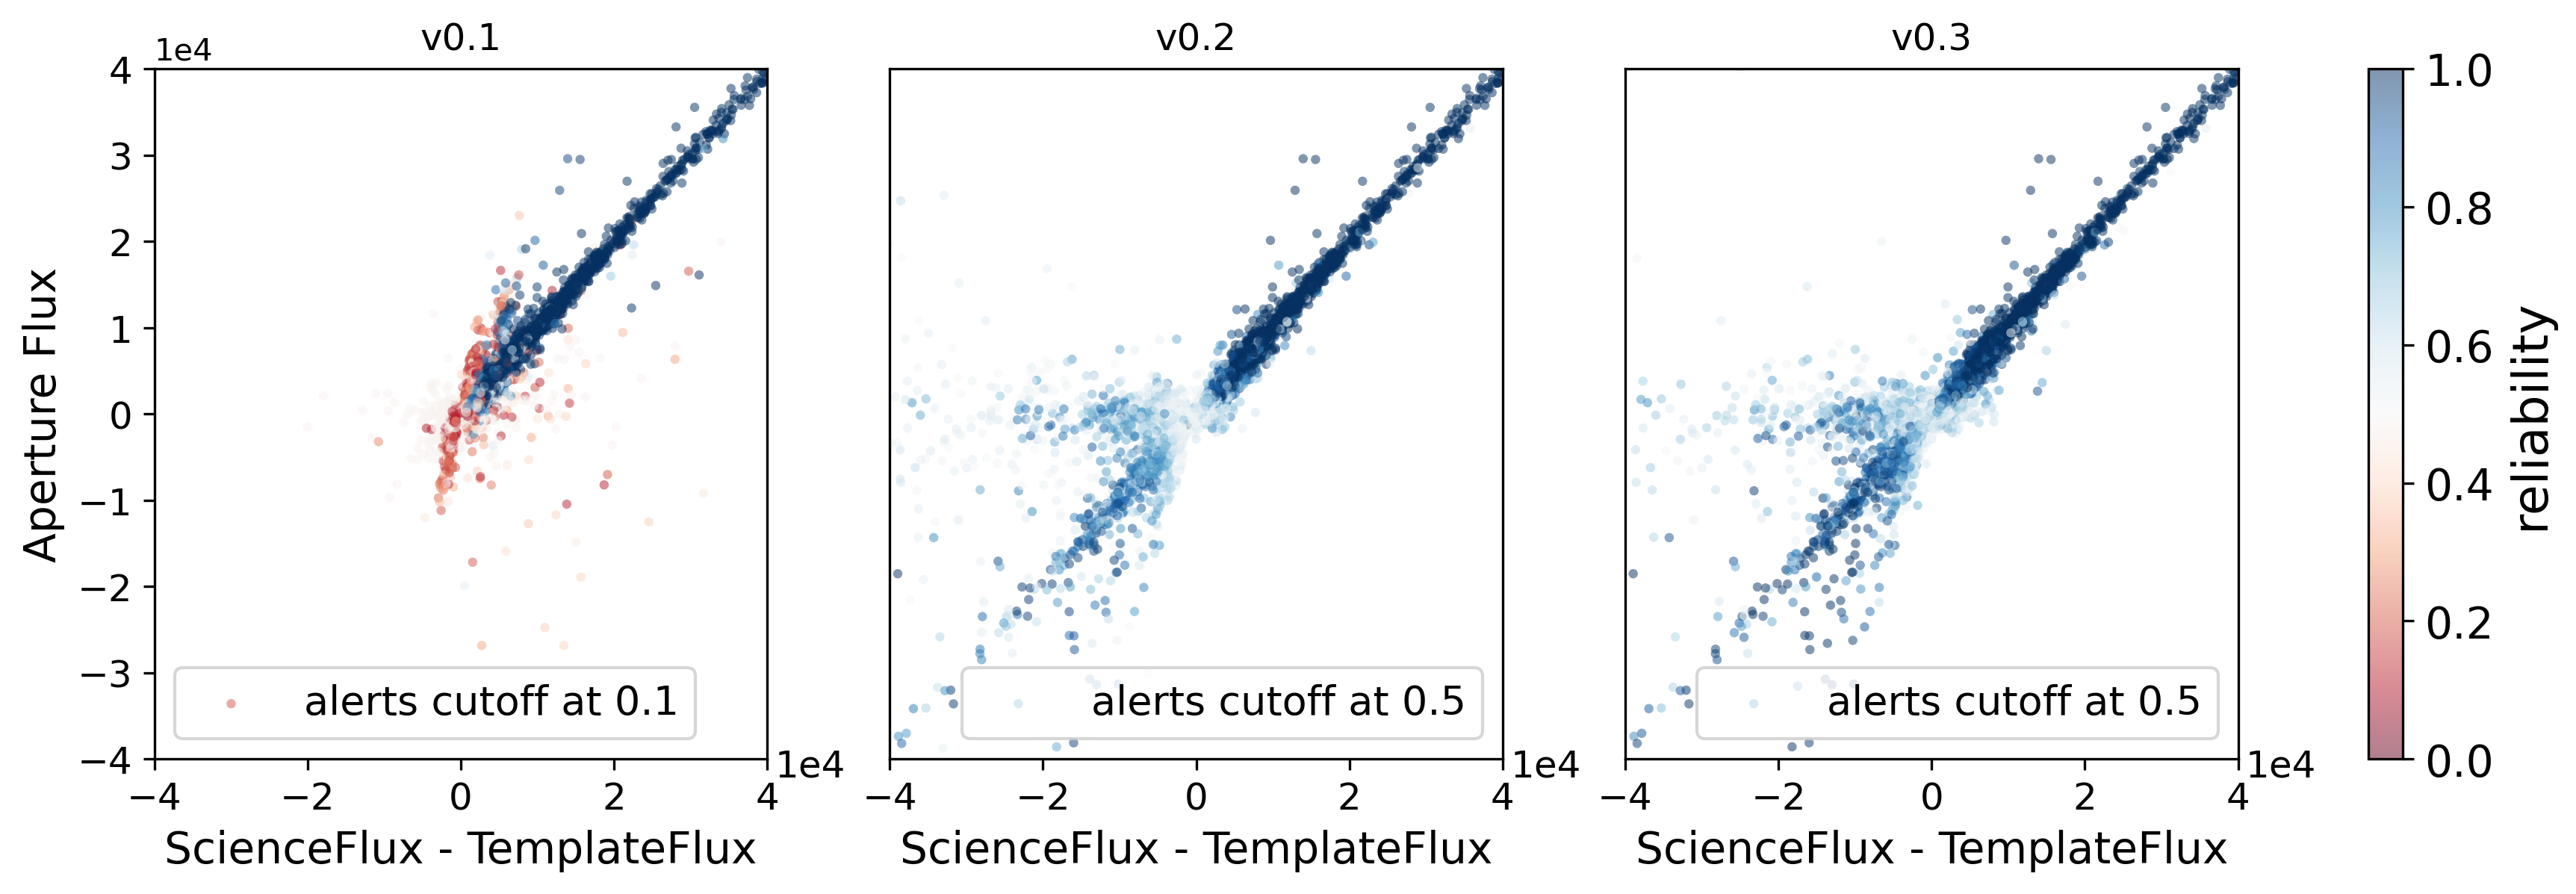
\includegraphics[width=1\linewidth]{figures/apflux_cutoff_version.png}
   \caption{DIA Aperture Flux vs ScienceFlux - TemplateFlux colored by the reliability score with a cutoff for each model version for a random set of DIA sources.}
    \label{fig:st_apflux_cutoff}
\end{figure}



\begin{figure}[htb!]
    \centering
    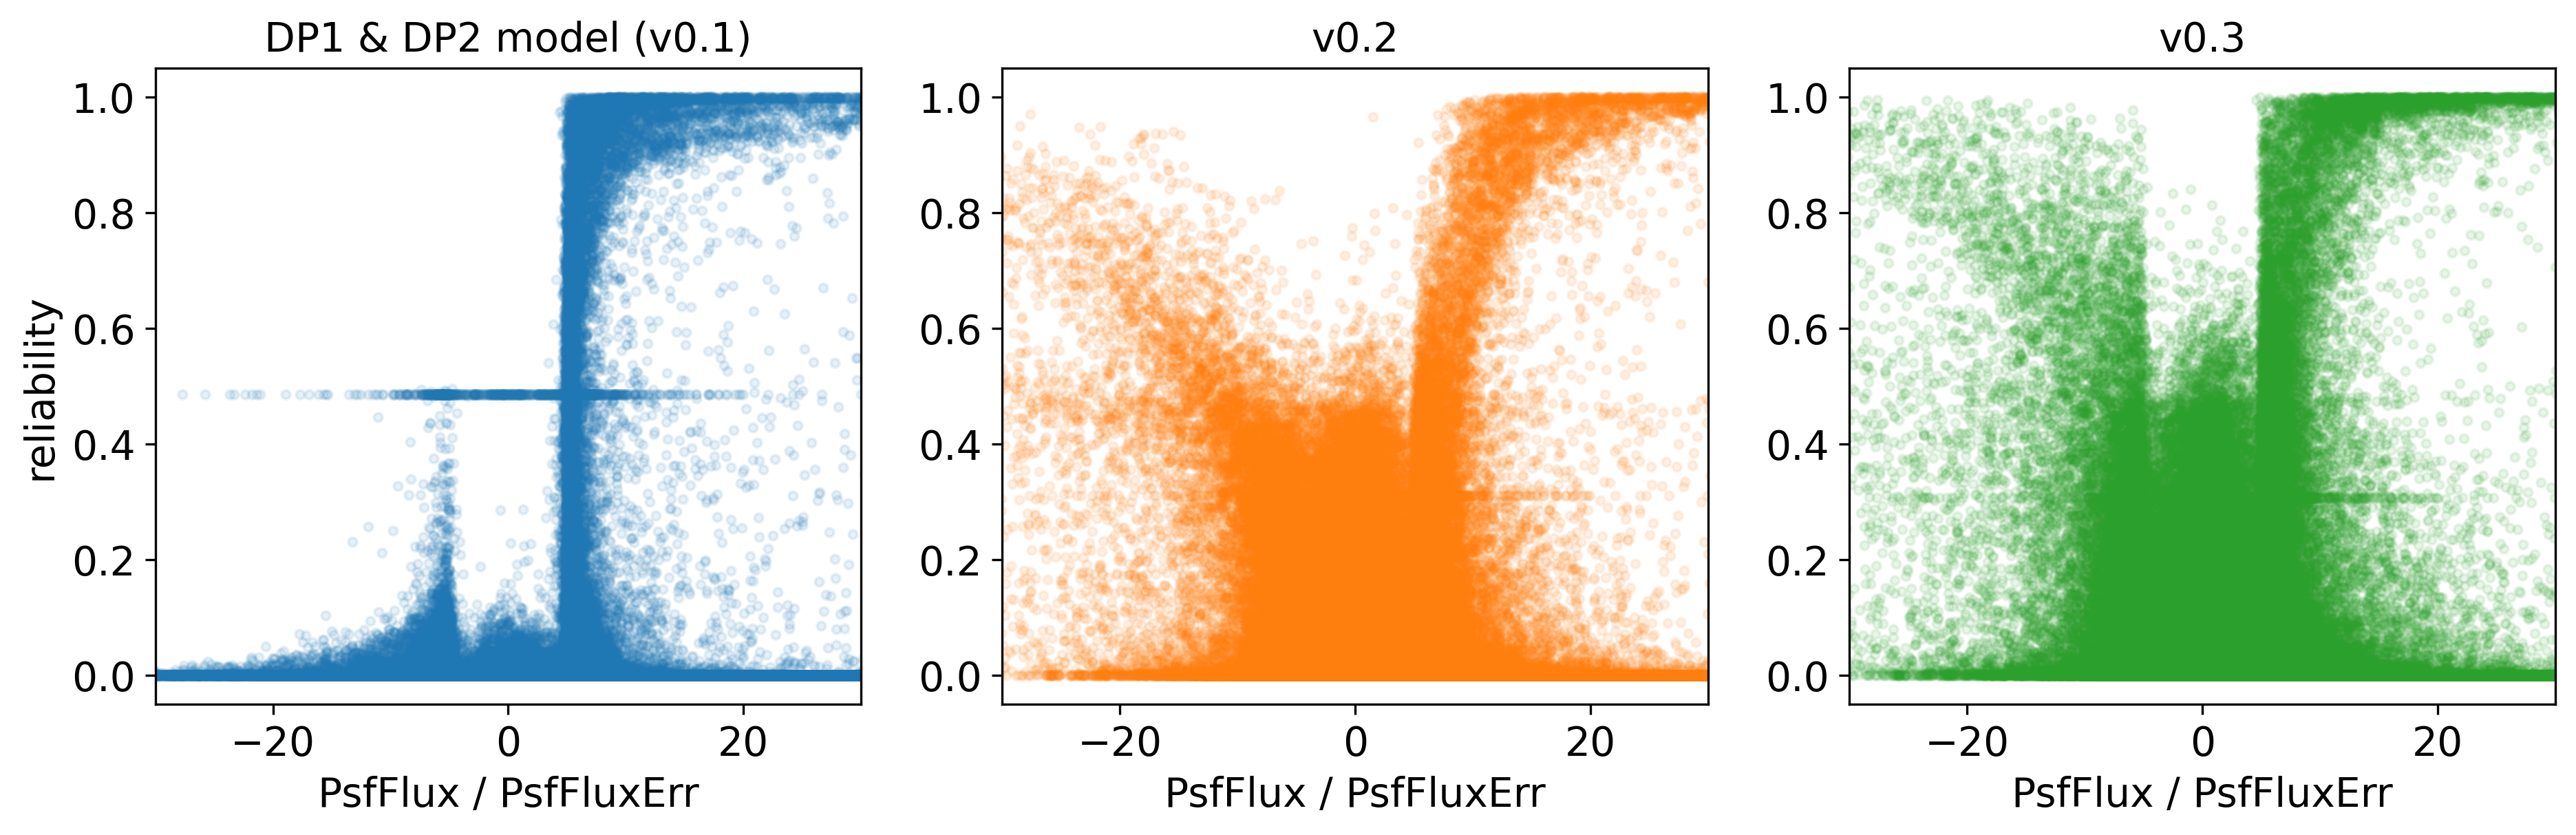
\includegraphics[width=1\linewidth]{figures/psf_psferr_version.png}
    \caption{\rel\ vs psfFlux/psfFluxErr for each model version for a random set of DIA sources.}
    \label{fig:psf/psferr_rel}
\end{figure}


The ratio of the quantity \texttt{psfFlux} (Flux for Point Source model) and the respective error (\texttt{psfFluxErr}), against the reliability score for each model, is shown in \autoref{fig:psf/psferr_rel}. In general, DIA sources with large psfFlux error have a reliability score smaller than $\sim 0.5$. For the \V1 model, where DIA sources with negative flux were not considered as part of the training set, the model assigned to all DIA sources with negative flux values a reliability score  $\rel<0.5$. The \rel\ in \V3 shows a less obvious functional dependence on the ratio of \texttt{psfFlux} to its error; sources in the region $-5\lesssim\texttt{psfFlux}/\texttt{psfFluxErr}\lesssim5$ are unlitley to get $\rel>0.6$, but sources with values up to this region result in any value of \rel, while in \V2 sources with $\texttt{psfFlux}/\texttt{psfFluxErr} \lesssim -5$ were less likely to result in high \rel\ scores with a visible direct correlation of \rel, with $|\texttt{psfFlux}/\texttt{psfFluxErr}|$. This effect is likely related to the diminished dependence of \rel\ on SNR, as described above.

% \begin{figure}[htb!]
%     \centering
%     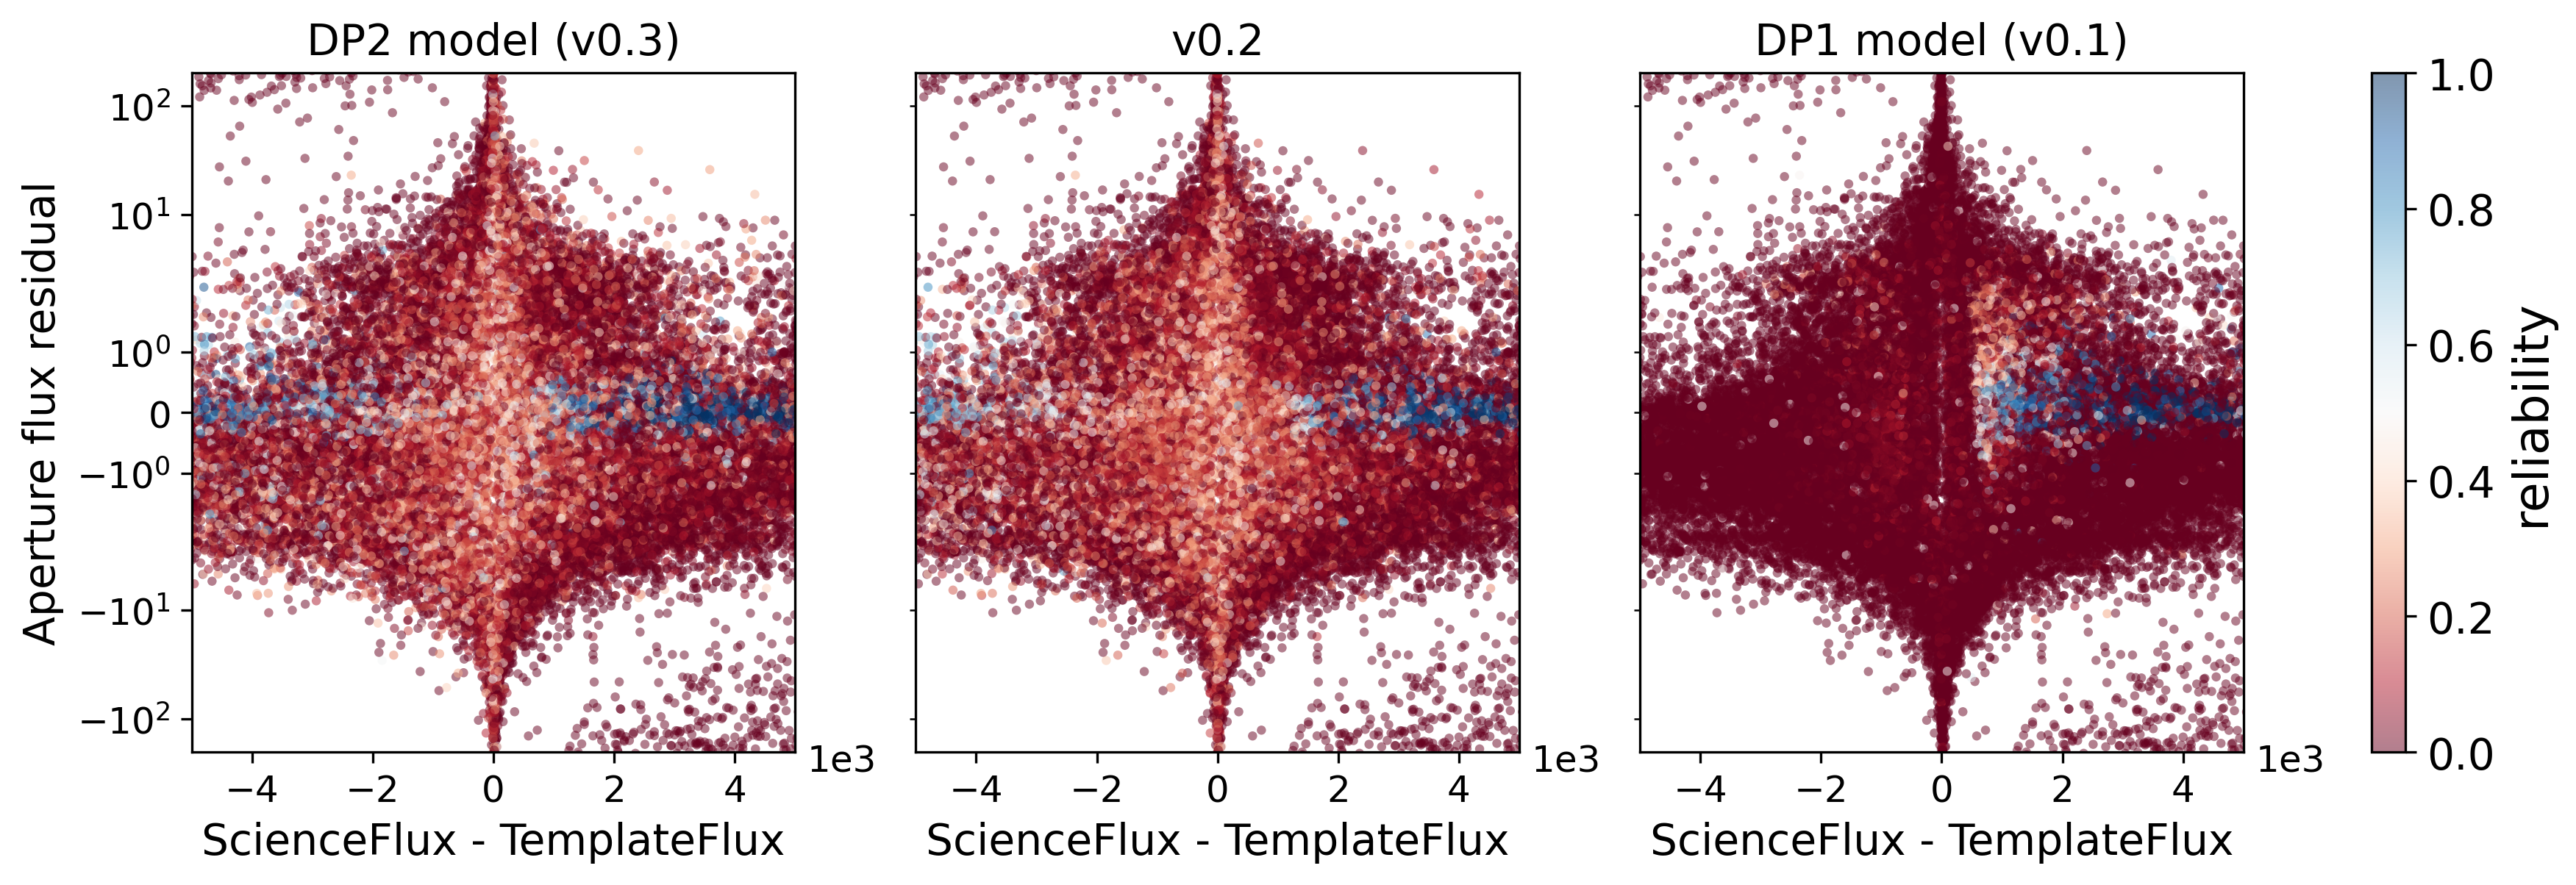
\includegraphics[width=1\linewidth]{figures/apfluxresidual_version.png}
%      \caption{ScienceFlux - TemplateFlux vs Aperture Flux residual colored by the reliability score for each model version}
%     \label{fig:st_apflux_res}
% \end{figure}

% \begin{figure}[htb!]
%     \centering
%     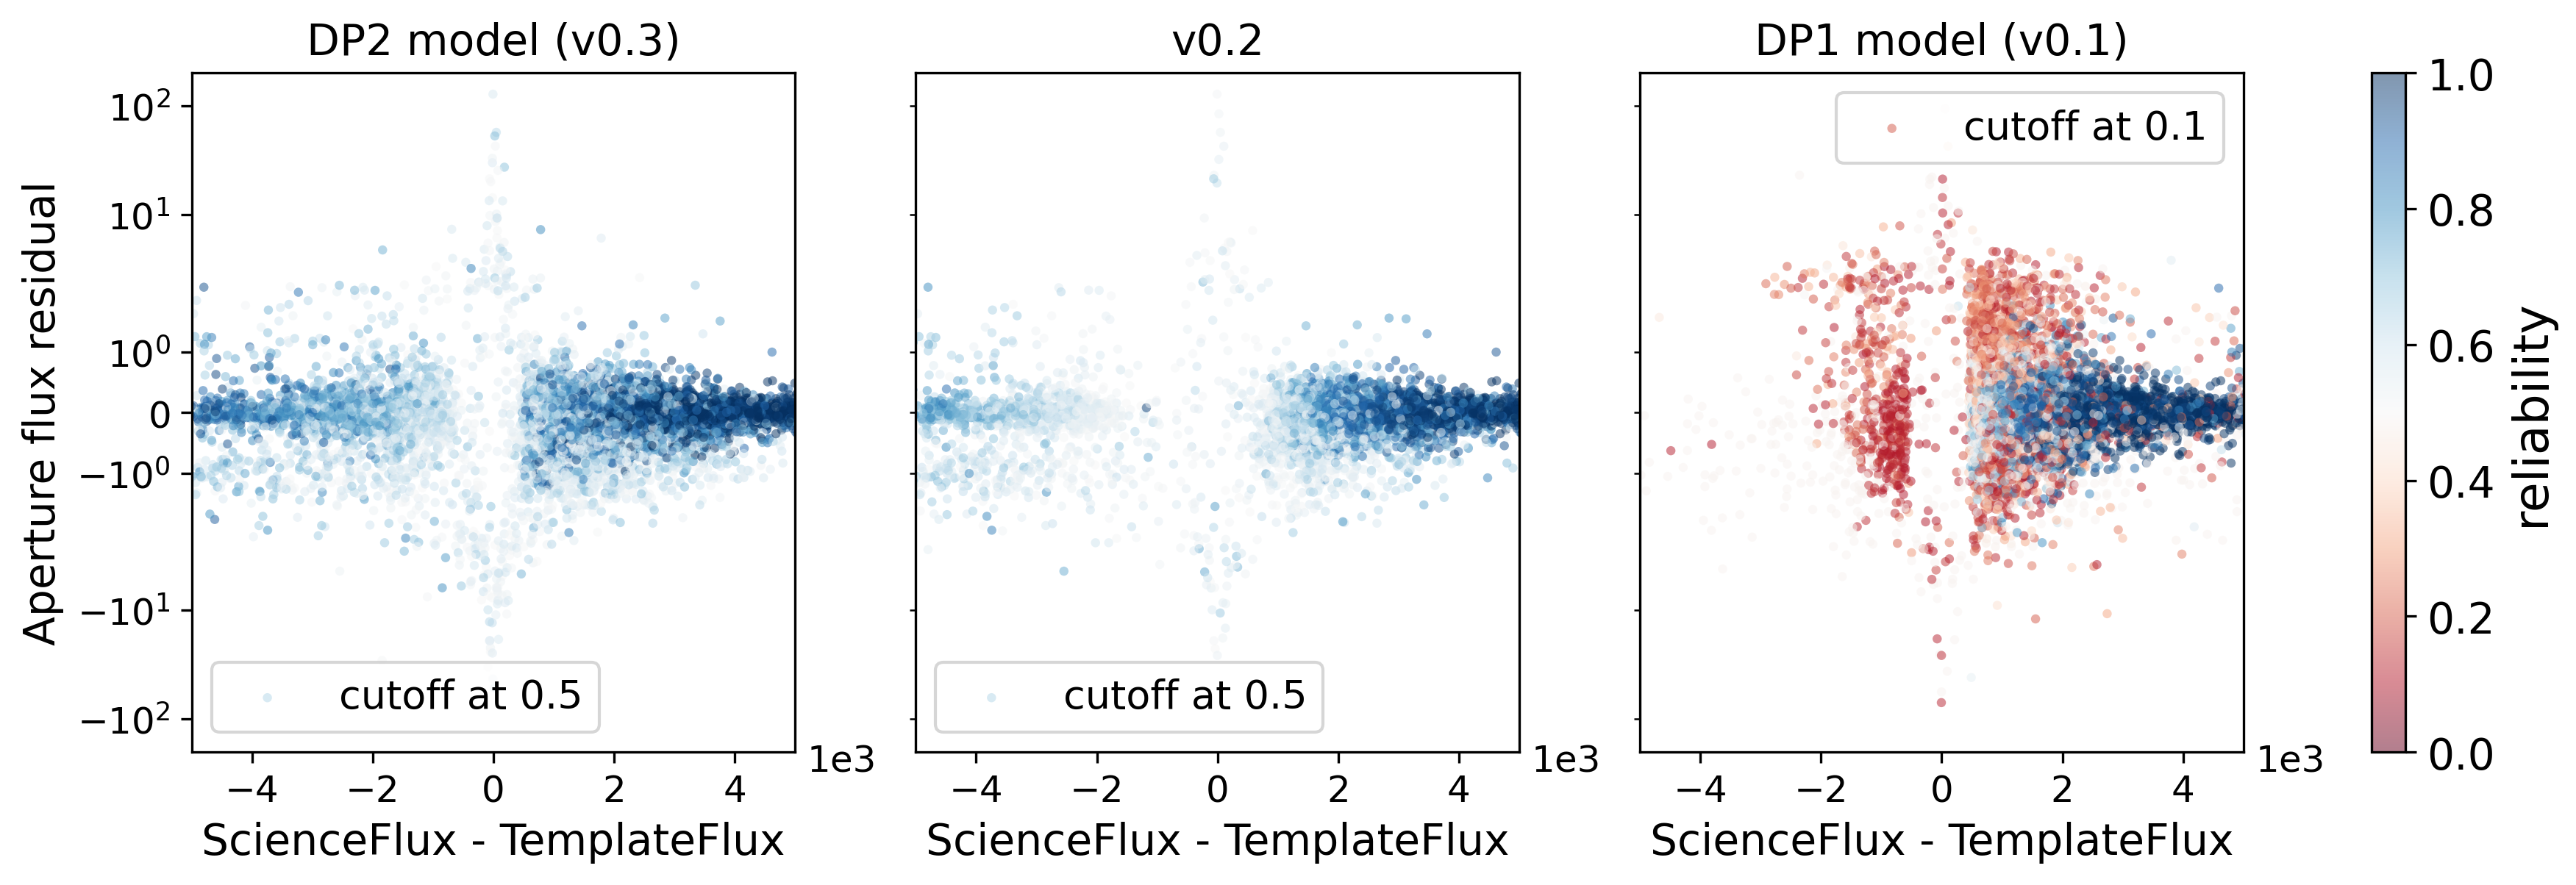
\includegraphics[width=1\linewidth]{figures/apfluxresidual_cutoff_version.png}
%     \caption{ScienceFlux - TemplateFlux vs Aperture Flux residual colored by the reliability score with a cutoff for each model version}
%     \label{fig:st_apflux_res_cutoff}
% \end{figure}

A quantitative assessment of the performance of each version of the Rubin ML-Reliability model is reported in the following sections.

\subsection{Model \V1 (deployed on DP1)}\label{sec:v01}
Throughout, the performance of the models is measured on all DIA sources, i.e., on any DIA detection with SNR>5 (while the LSST requirements are set to SNR=6).

The \V1 model was deployed on DP1 data. The model had achieved a purity of 98.90\% and completeness of 97.00\% on the test dataset generated from the same collection from which the training and validation data were produced (DC2 simulations, LSSTComCam images with and without injections, see \autoref{sec:data}).
On a separate LSSTComCam test set, where \texttt{Reals} are comprised entirely of injections, the model achieved an accuracy of 98.06\%, purity
of 97.87\%, and completeness of 98.27\%, meeting construction requirements. %The weights up to this point were the ones used to generate the reliability score on DP1 data \cite[DP1]{RTN-095}. 

To further assess the model performance, we used a dataset of fakes injections into the COSMOS field LSSTCam images, which we hereafter refer to as `COSMOS injections'. This dataset is completely separated and generated independently of the training data set (\autoref{tab:list_data}). The performance of \V1 on this dataset is shown in \autoref{fig:cosmos_dp1}. A purity and completeness of 87\% are achieved at a threshold of \rel=0.907.

\begin{figure}
    \centering
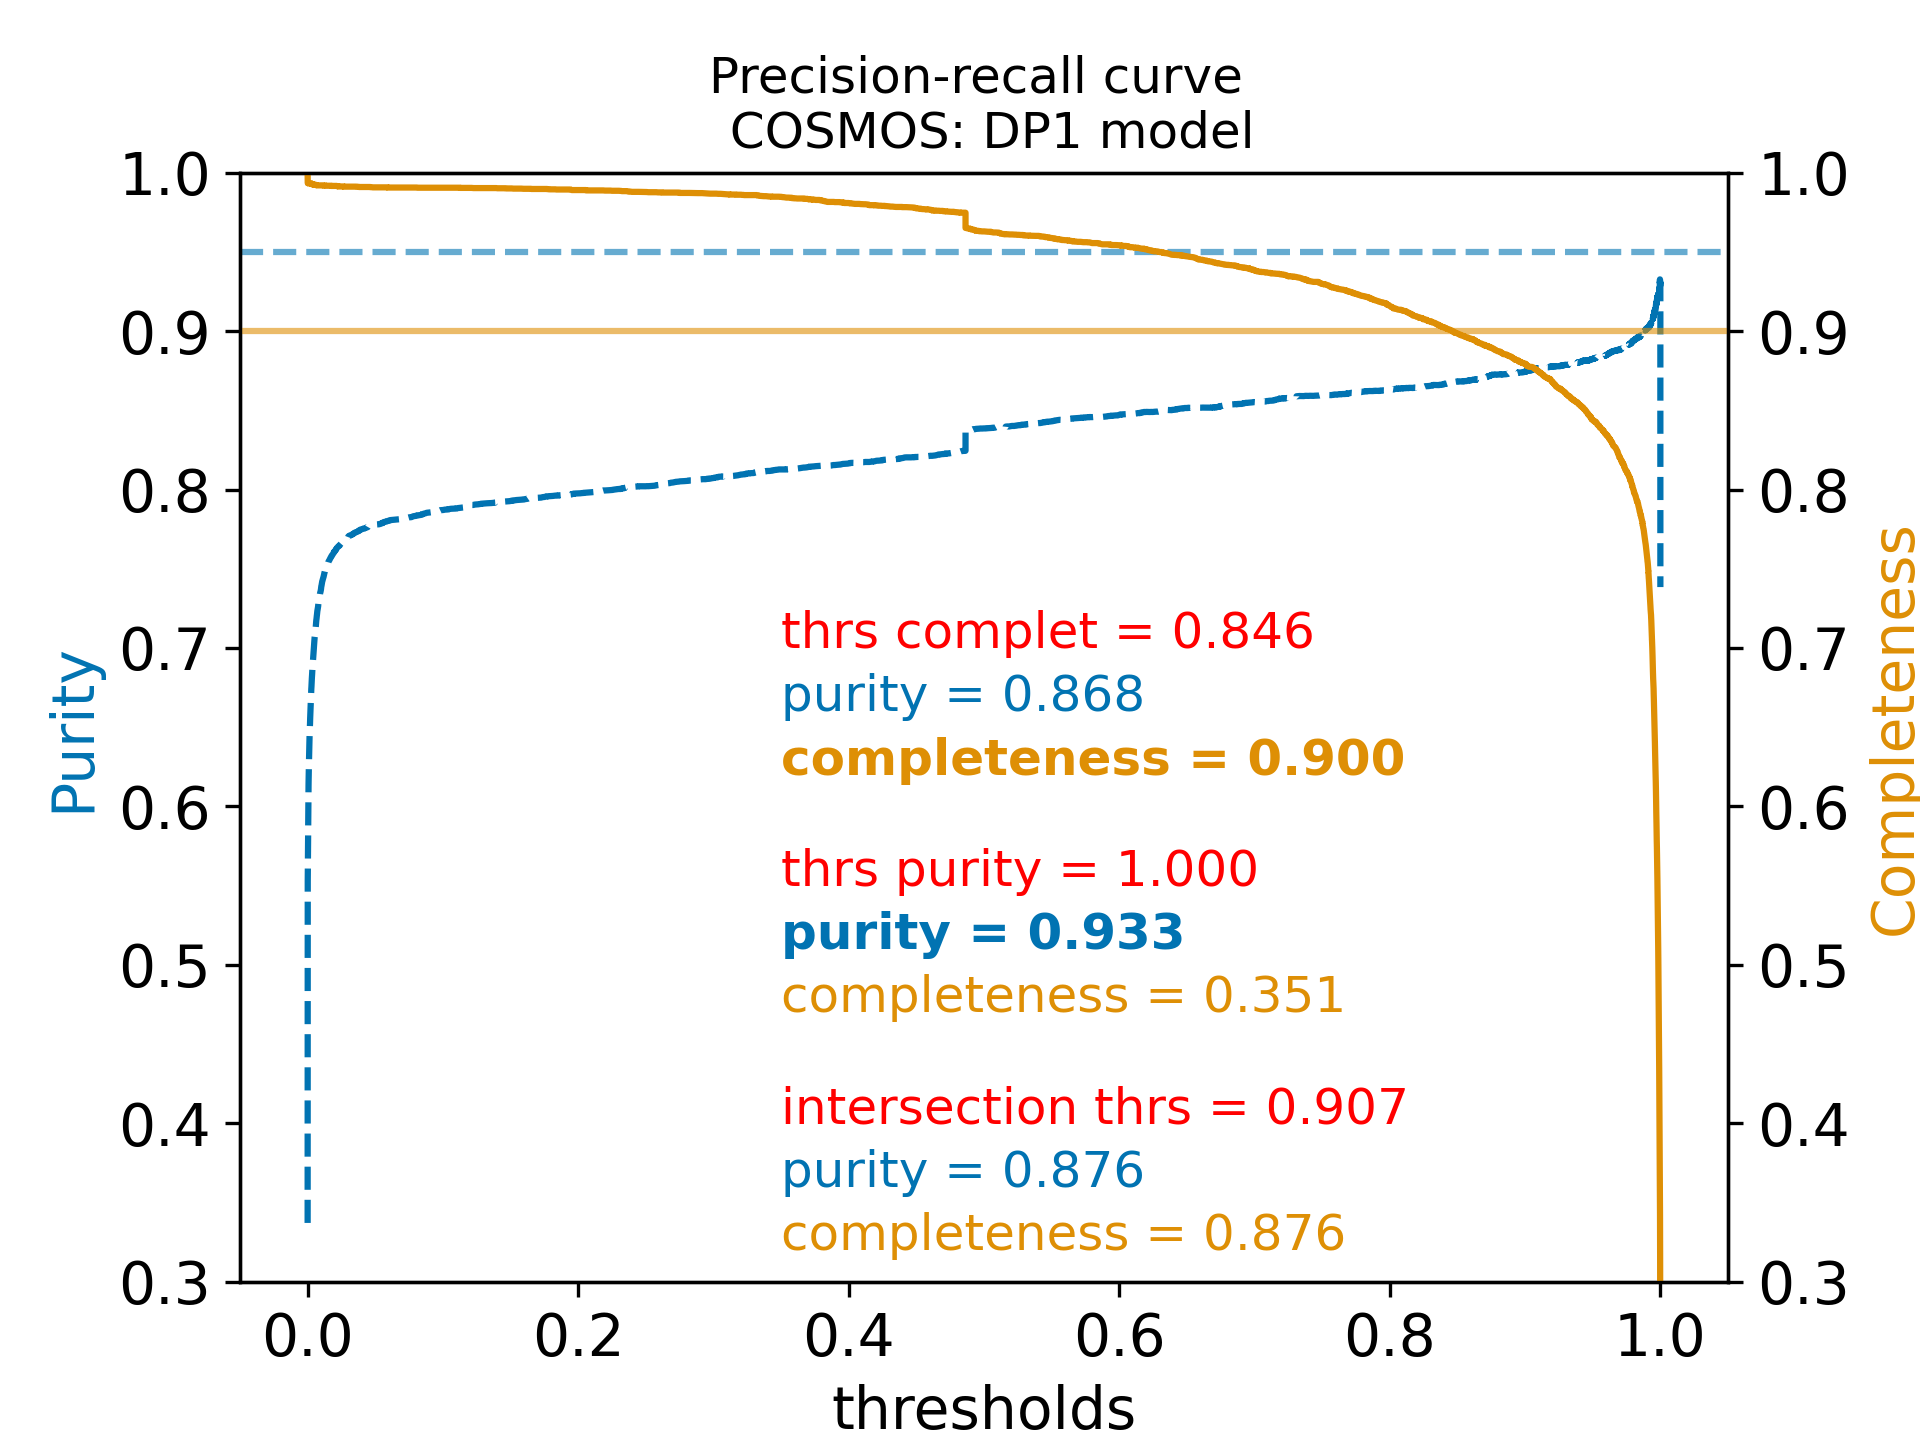
\includegraphics[width=0.6\linewidth]{figures/cosmos_dp1_model.png}
    \caption{Performance of the \V1 (DP1) model on fake sources injected into the COSMOS field LSSTCam images.}
    \label{fig:cosmos_dp1}
\end{figure}


As reported in \cite[DP1]{RTN-095}, and shown in \autoref{tab:classification_results_dp1}, when tested on real LSSTComCam detection generated by cross-matching DIA sources as discussed in \autoref{sec:data}, and after applying a threshold of \rel=0.5, the purity and completeness achieved on Solar System detections is high, on transient detections completeness is $\sim75\%$, but completeness is very low on variable stars. Since variable stars were not included in the training dataset, and they have specific complexities for DIA in the subtraction of a PSF from an existing PSF (unlike transients and solar system detections), it is to be expected that the model would not perform well on this class. This motivated the development of the Zooniverse project.

\begin{table}[ht]
\centering
\caption{Classification Results for Solar System Transient and Variable objects using the DP1 model with a reliability threshold of 0.5.}
\label{tab:classification_results_dp1}
\begin{tabular}{|c|c|c|c|}
\hline
\textbf{Type} & \textbf{True Positives} & \textbf{False Negatives} & \textbf{Total Objects} \\ \hline
SS & 93.5\% & 6.5\% & 5988 \\ \hline
Transients & 73.7\% & 26.3\% & 99 \\ \hline
Variables & 3.5\% & 96.5\% & 316 \\ \hline
\end{tabular}
\end{table}



\subsection{Model \V2 deployed on initial alerts}

The \V2 was deployed on the initial LSST alerts (February 2026). The \V2 model was tested against the COSMOS injections. Results are shown in \autoref{fig:cosmos_v02}.

\begin{figure}
    \centering
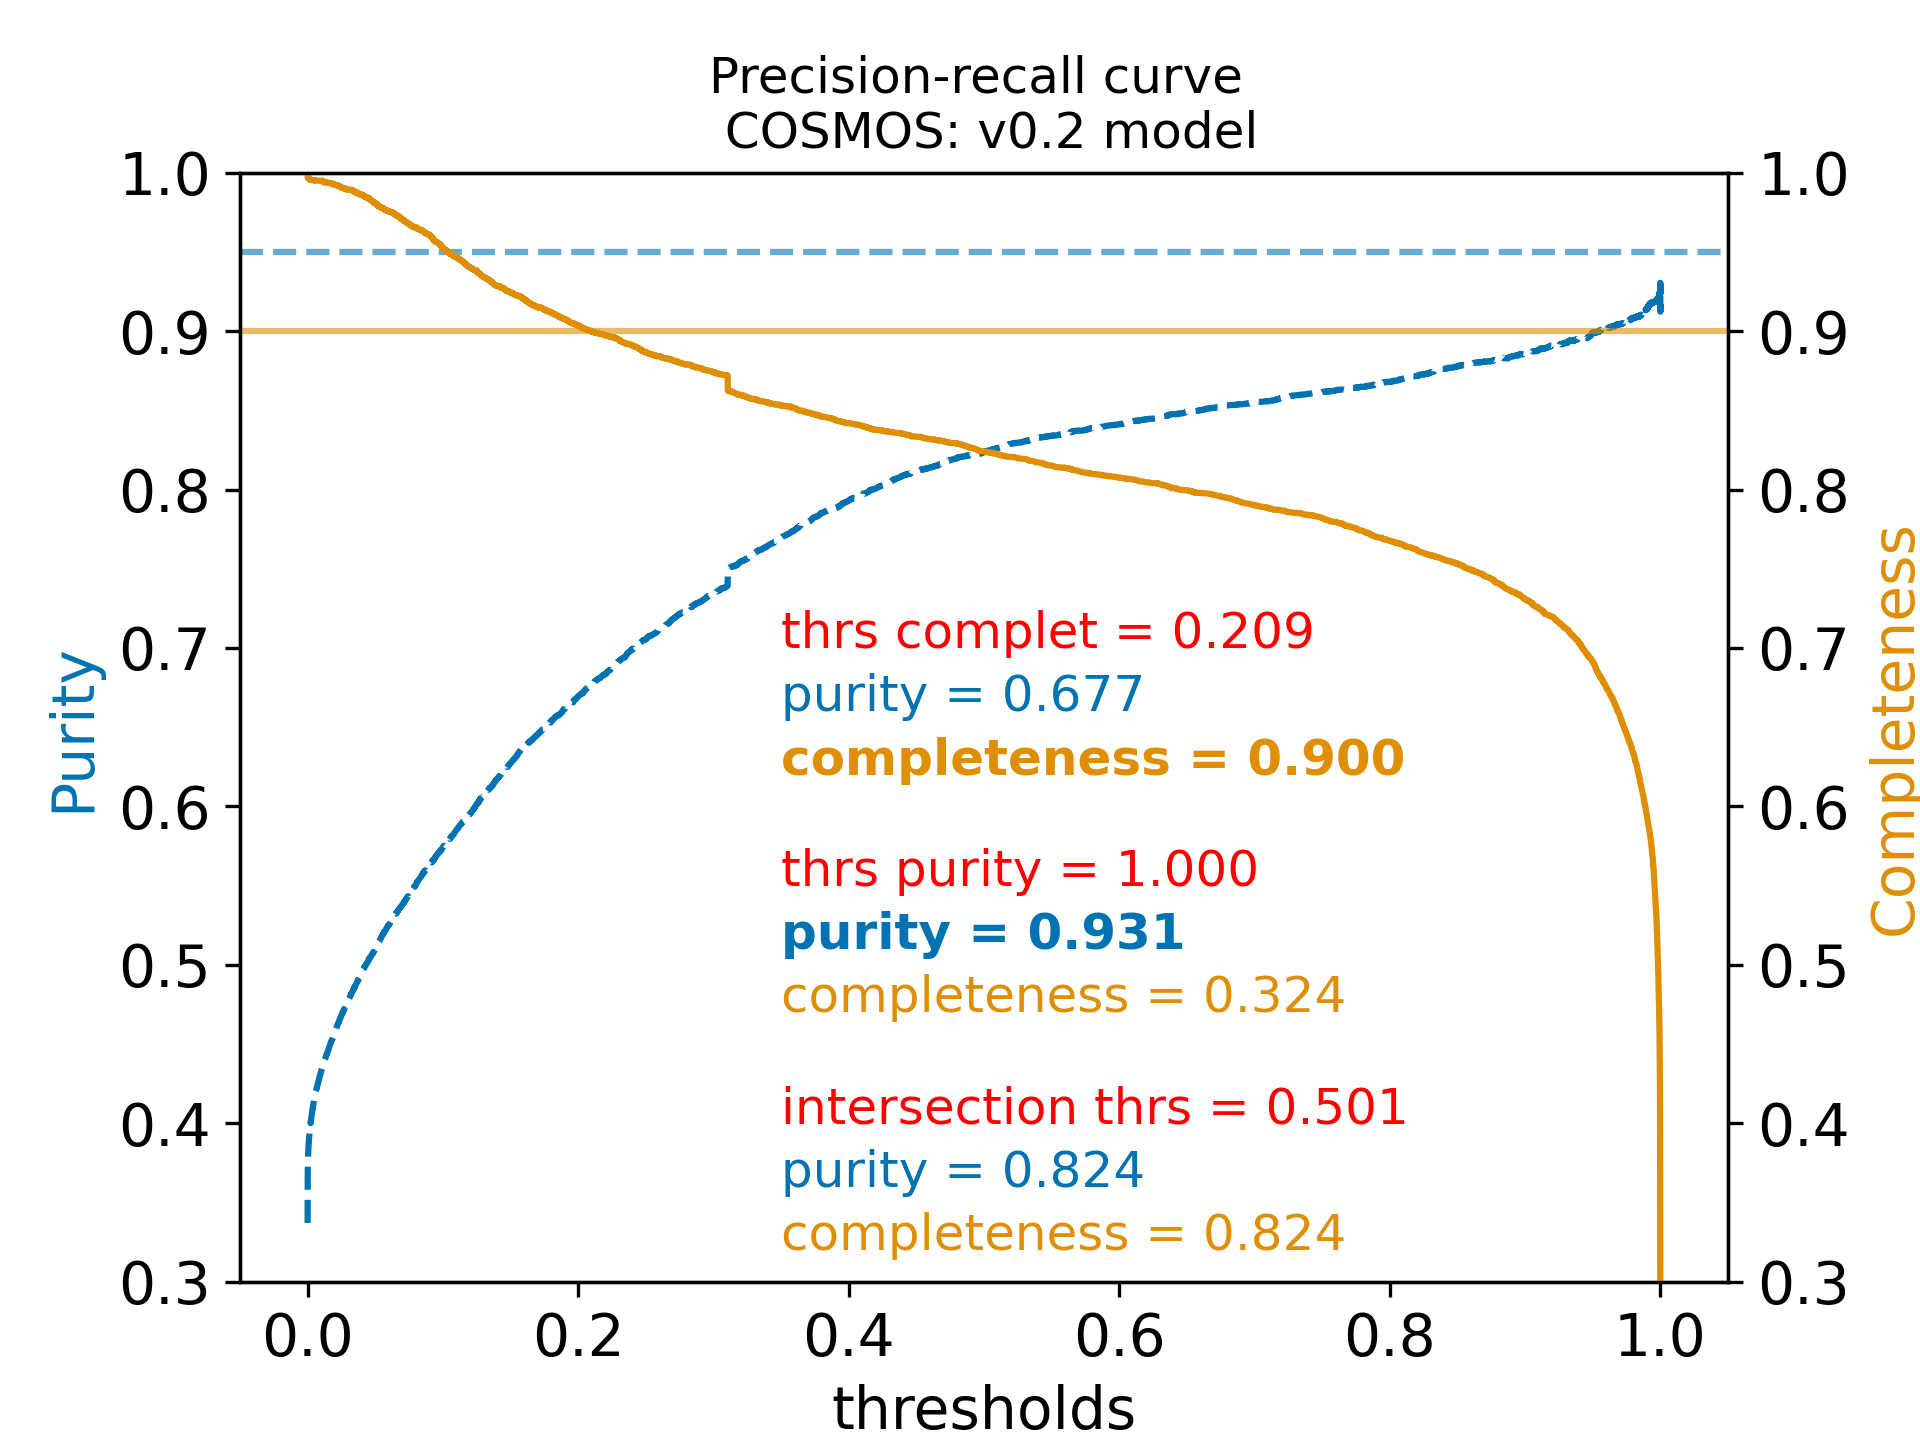
\includegraphics[width=0.6\linewidth]{figures/cosmos_v02_model.png}
    \caption{Performance of the \V2 model on fake sources injected into the COSMOS field LSSTCam images.}
    \label{fig:cosmos_v02}
\end{figure}


The optimal balance of purity and completeness is achieved at \rel=0.501 (82\% purity and 82\%  completeness).

\subsection{Model \V3 (deployed on DP2)}

Model \V3 was benchmarked for processing DP2 data. 

\begin{figure*}[htb!]
   \centering
   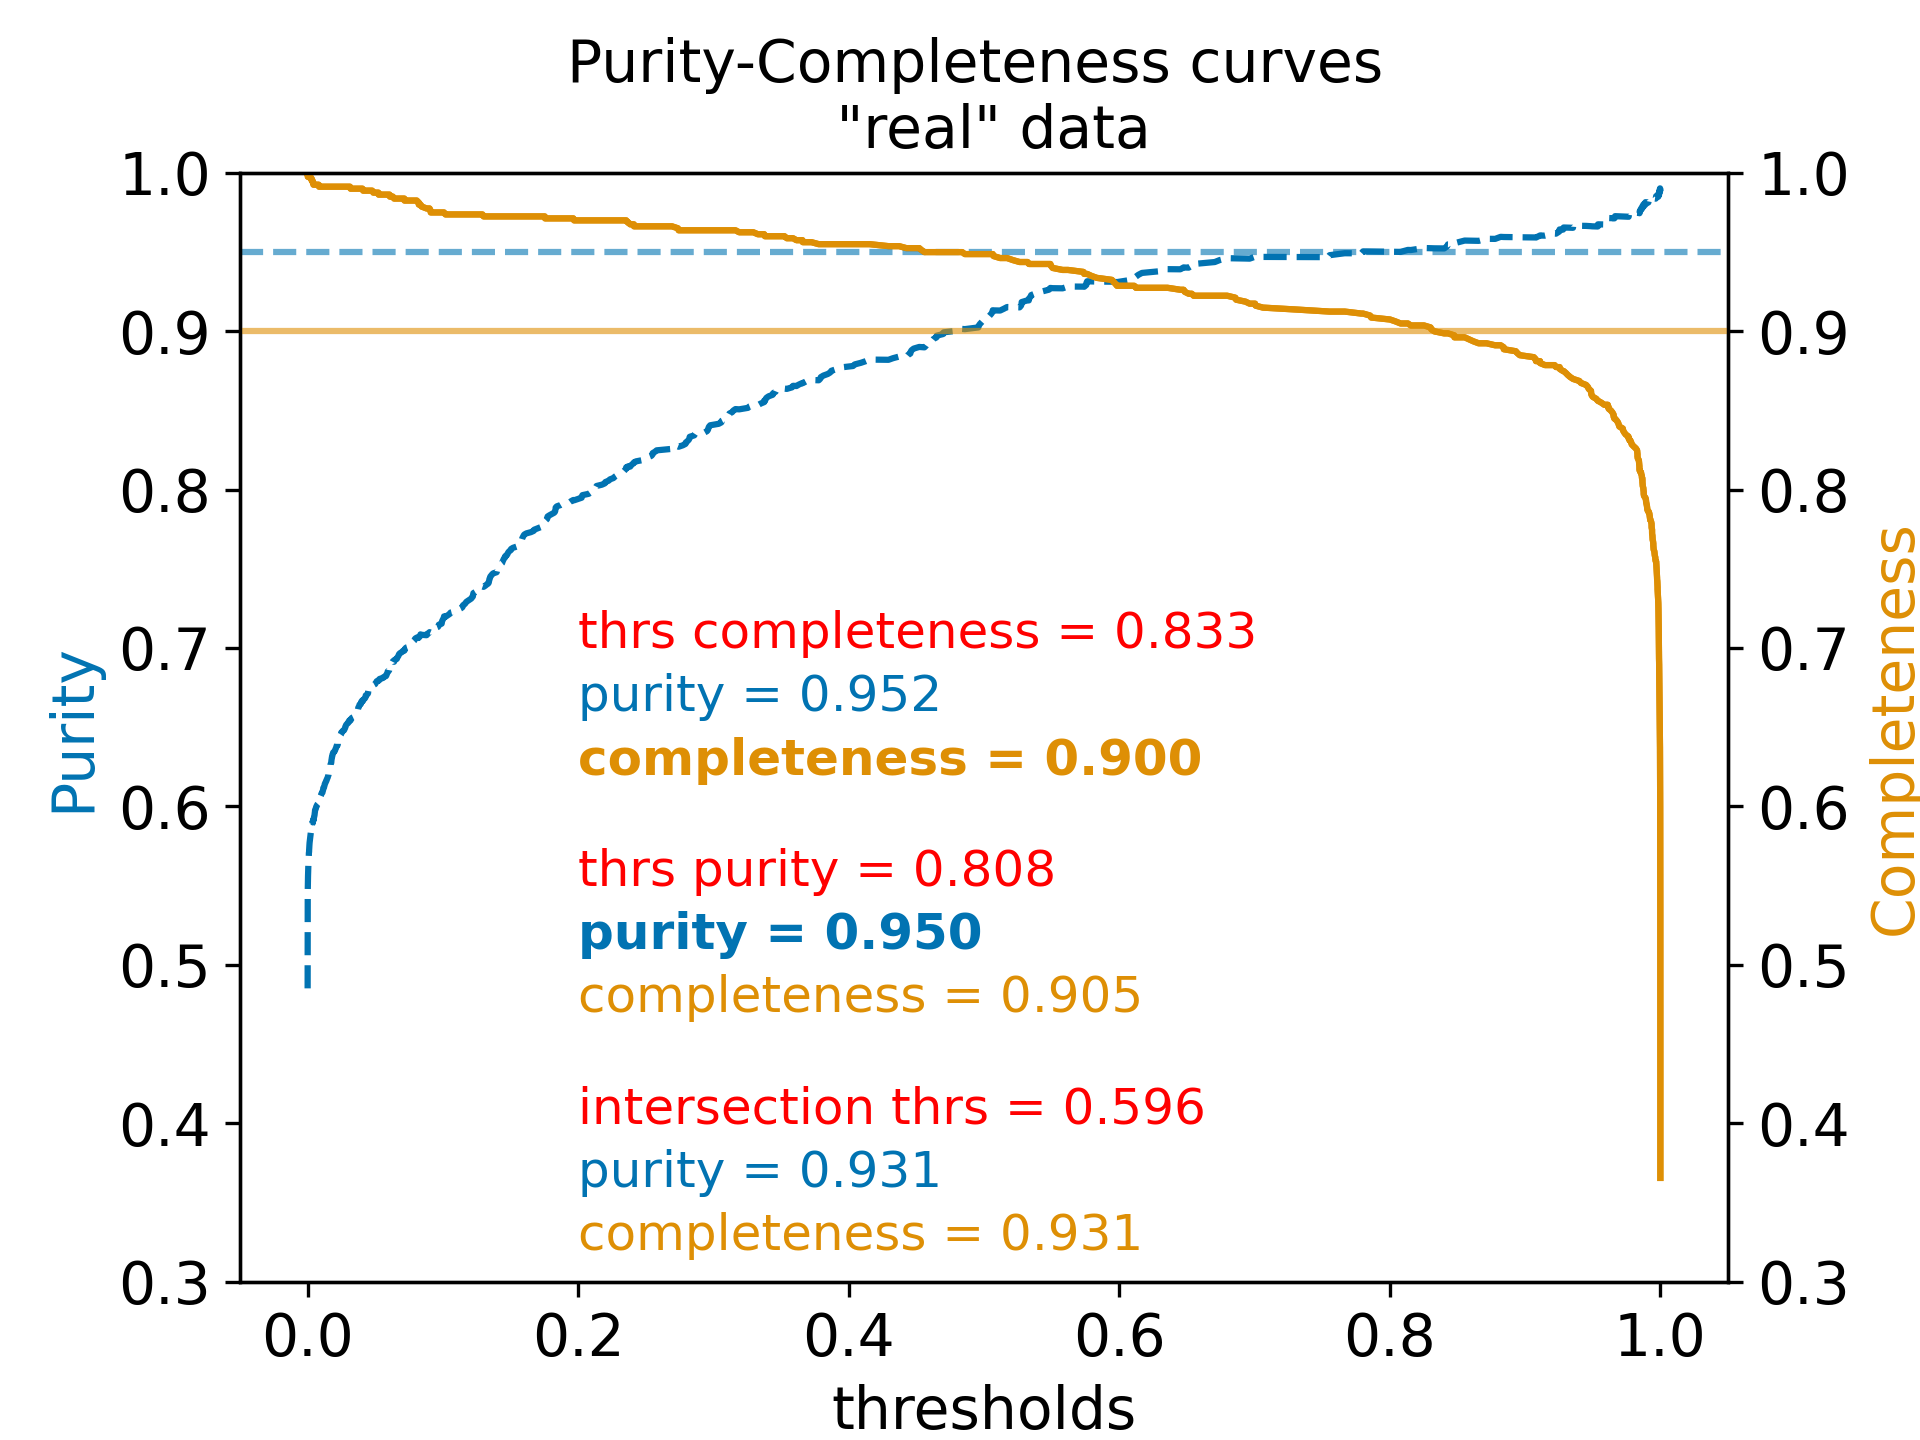
\includegraphics[width=0.45\linewidth]{figures/stable_dp2_report_new_model.png}
    \includegraphics[width=0.45\linewidth]{figures/ComCam_dp2_report_new_model.png}
    \caption{Model \V3 Purity and Completeness curves. \textit{Left}: For the test data without fake injections (Zooniverse labels), at a threshold of 0.596, the purity (precision) and completeness (recall) are both 93.1\%. \textit{Right}: For the LSSTComCam fakes test data, at a threshold of 0.301, the purity (precision) and completeness (recall) are both 97.5\%. Users can choose their own reliability threshold to trade off completeness vs. purity.
}
\label{fig:dp2_performance}
\end{figure*}

In testing, the model reached a purity $\geq 95\%$ and completeness $\geq 90\%$ with threshold values $0.808 \leq$\rel $\leq 0.833$ on the test LSSTCam data without fake injections. On the LSSTComCam injections test set, the model reached a purity $\geq 95\%$ and completeness $\geq 90\%$, obtained with values $0.129 \leq $ \rel $\leq 0.899$. 
\autoref{fig:dp2_performance} shows the corresponding purity and completeness curves.

The \V3 model performance on the COSMOS injection is shown in \autoref{fig:cosmos_dp2}. 84\% Purity and 84\% Completeness are achieved at $\rel=0.785$.


\begin{figure}
    \centering
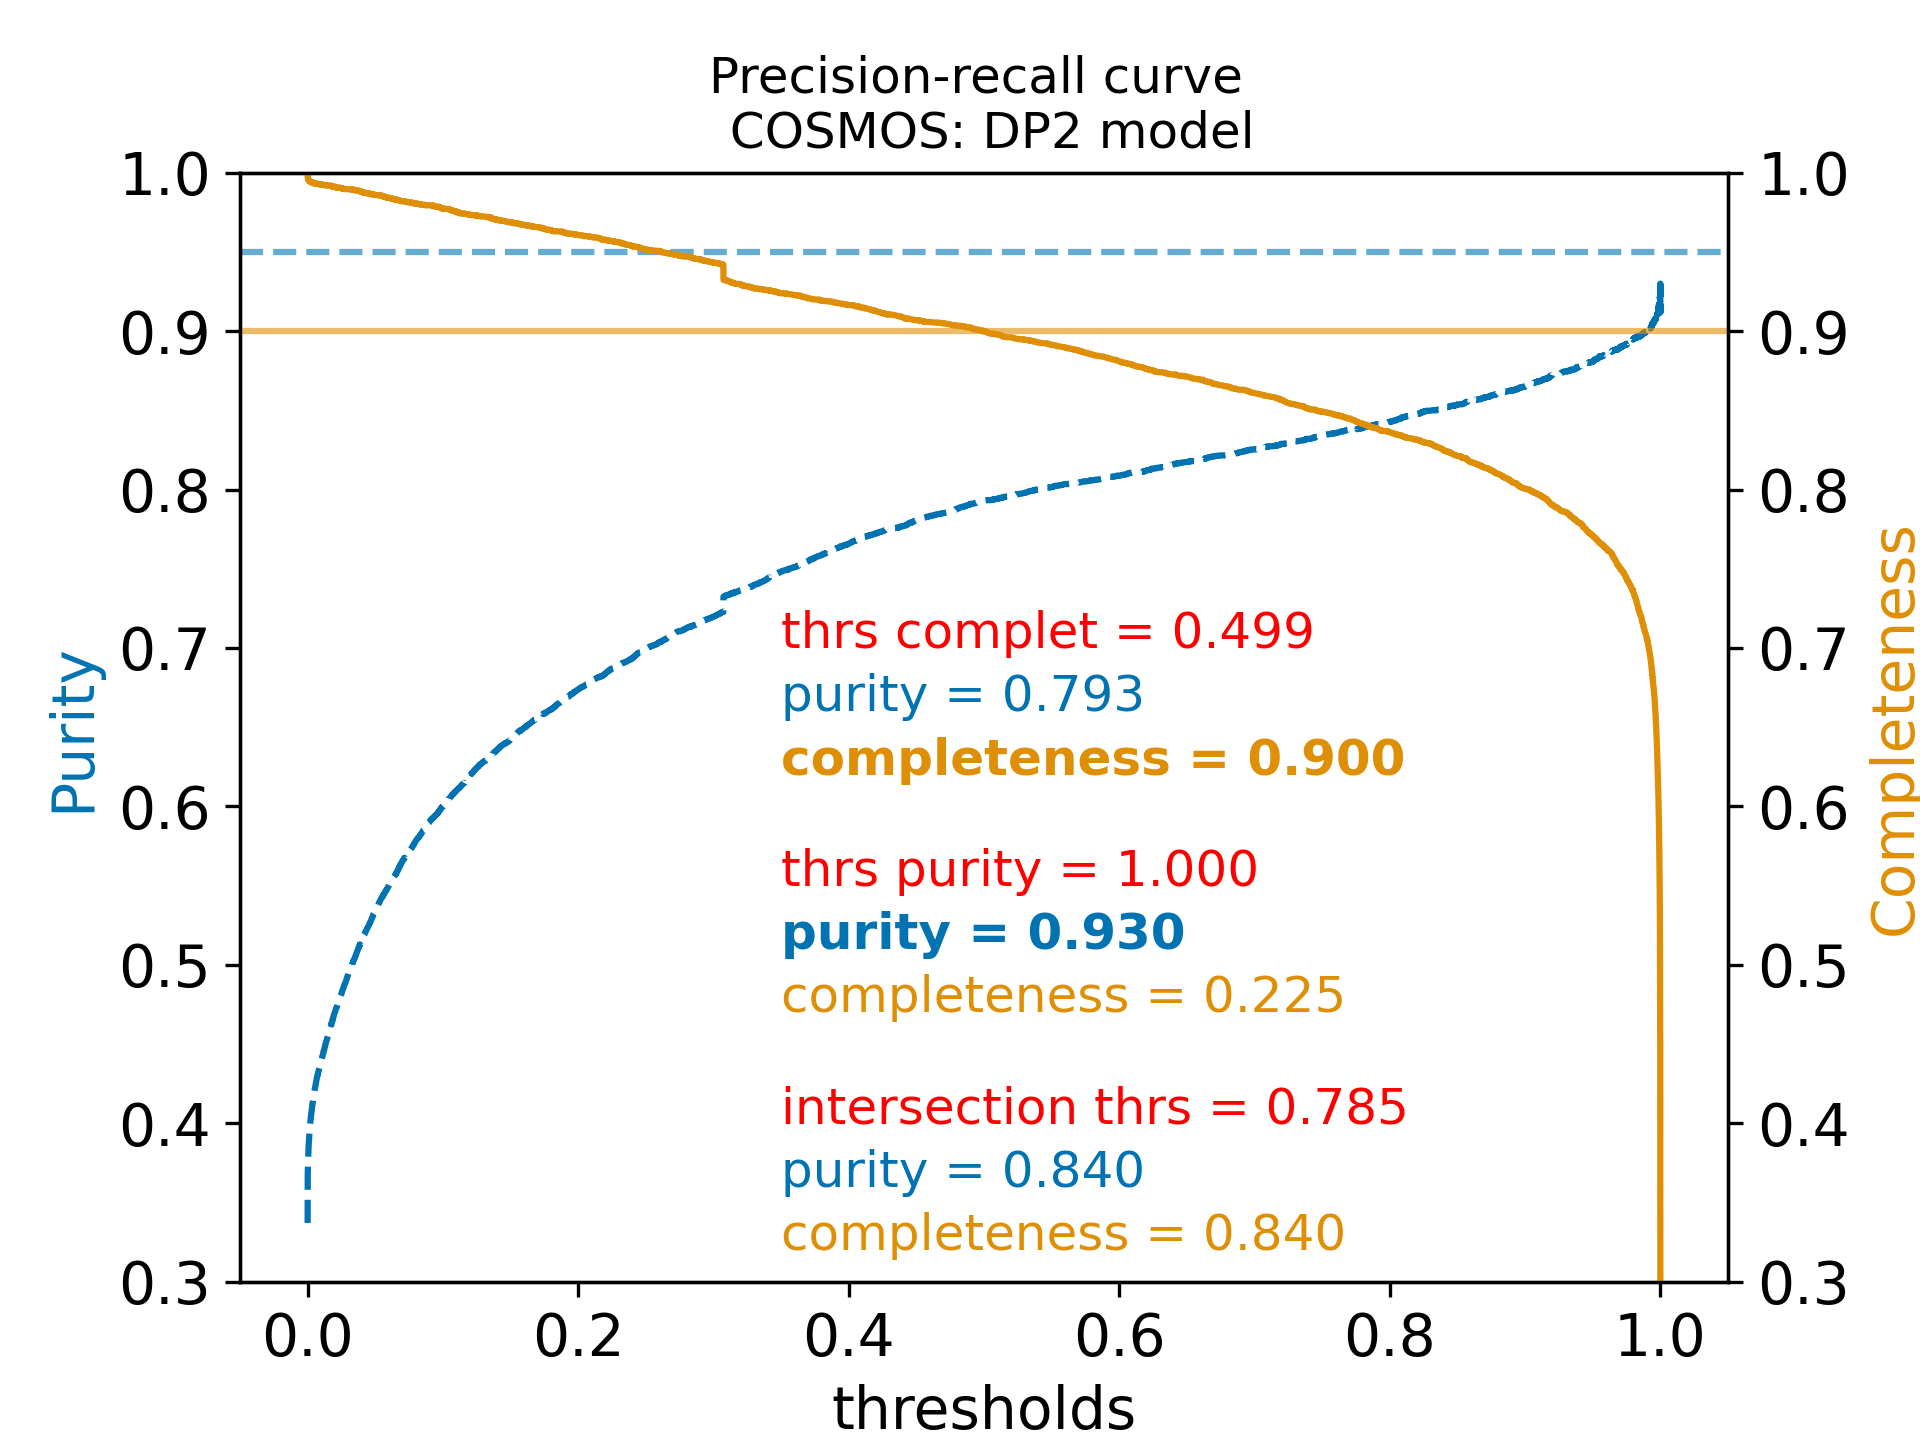
\includegraphics[width=0.6\linewidth]{figures/cosmos_dp2_report_new_model.png}
    \caption{Performance of the DP2 model on fake sources injected into the COSMOS field LSSTCam images.}
    \label{fig:cosmos_dp2}
\end{figure}


The distribution of \V3 \rel\ per data origin is shown in \autoref{fig:distribution_rel_score}.
Once again, we see that nearly all Solar System detection receive a $\rel\sim1$ score while the \rel\ for other data sources varies, with Gaia and the high confidence \V1 labels (`reliability\_cuts`) receiving generally low \rel.

The full Purity and Completeness curves per data origin as measured on the original test data are shown in \autoref{fig:dp2_performance_byset}.

\begin{figure}[htb!]
    \centering
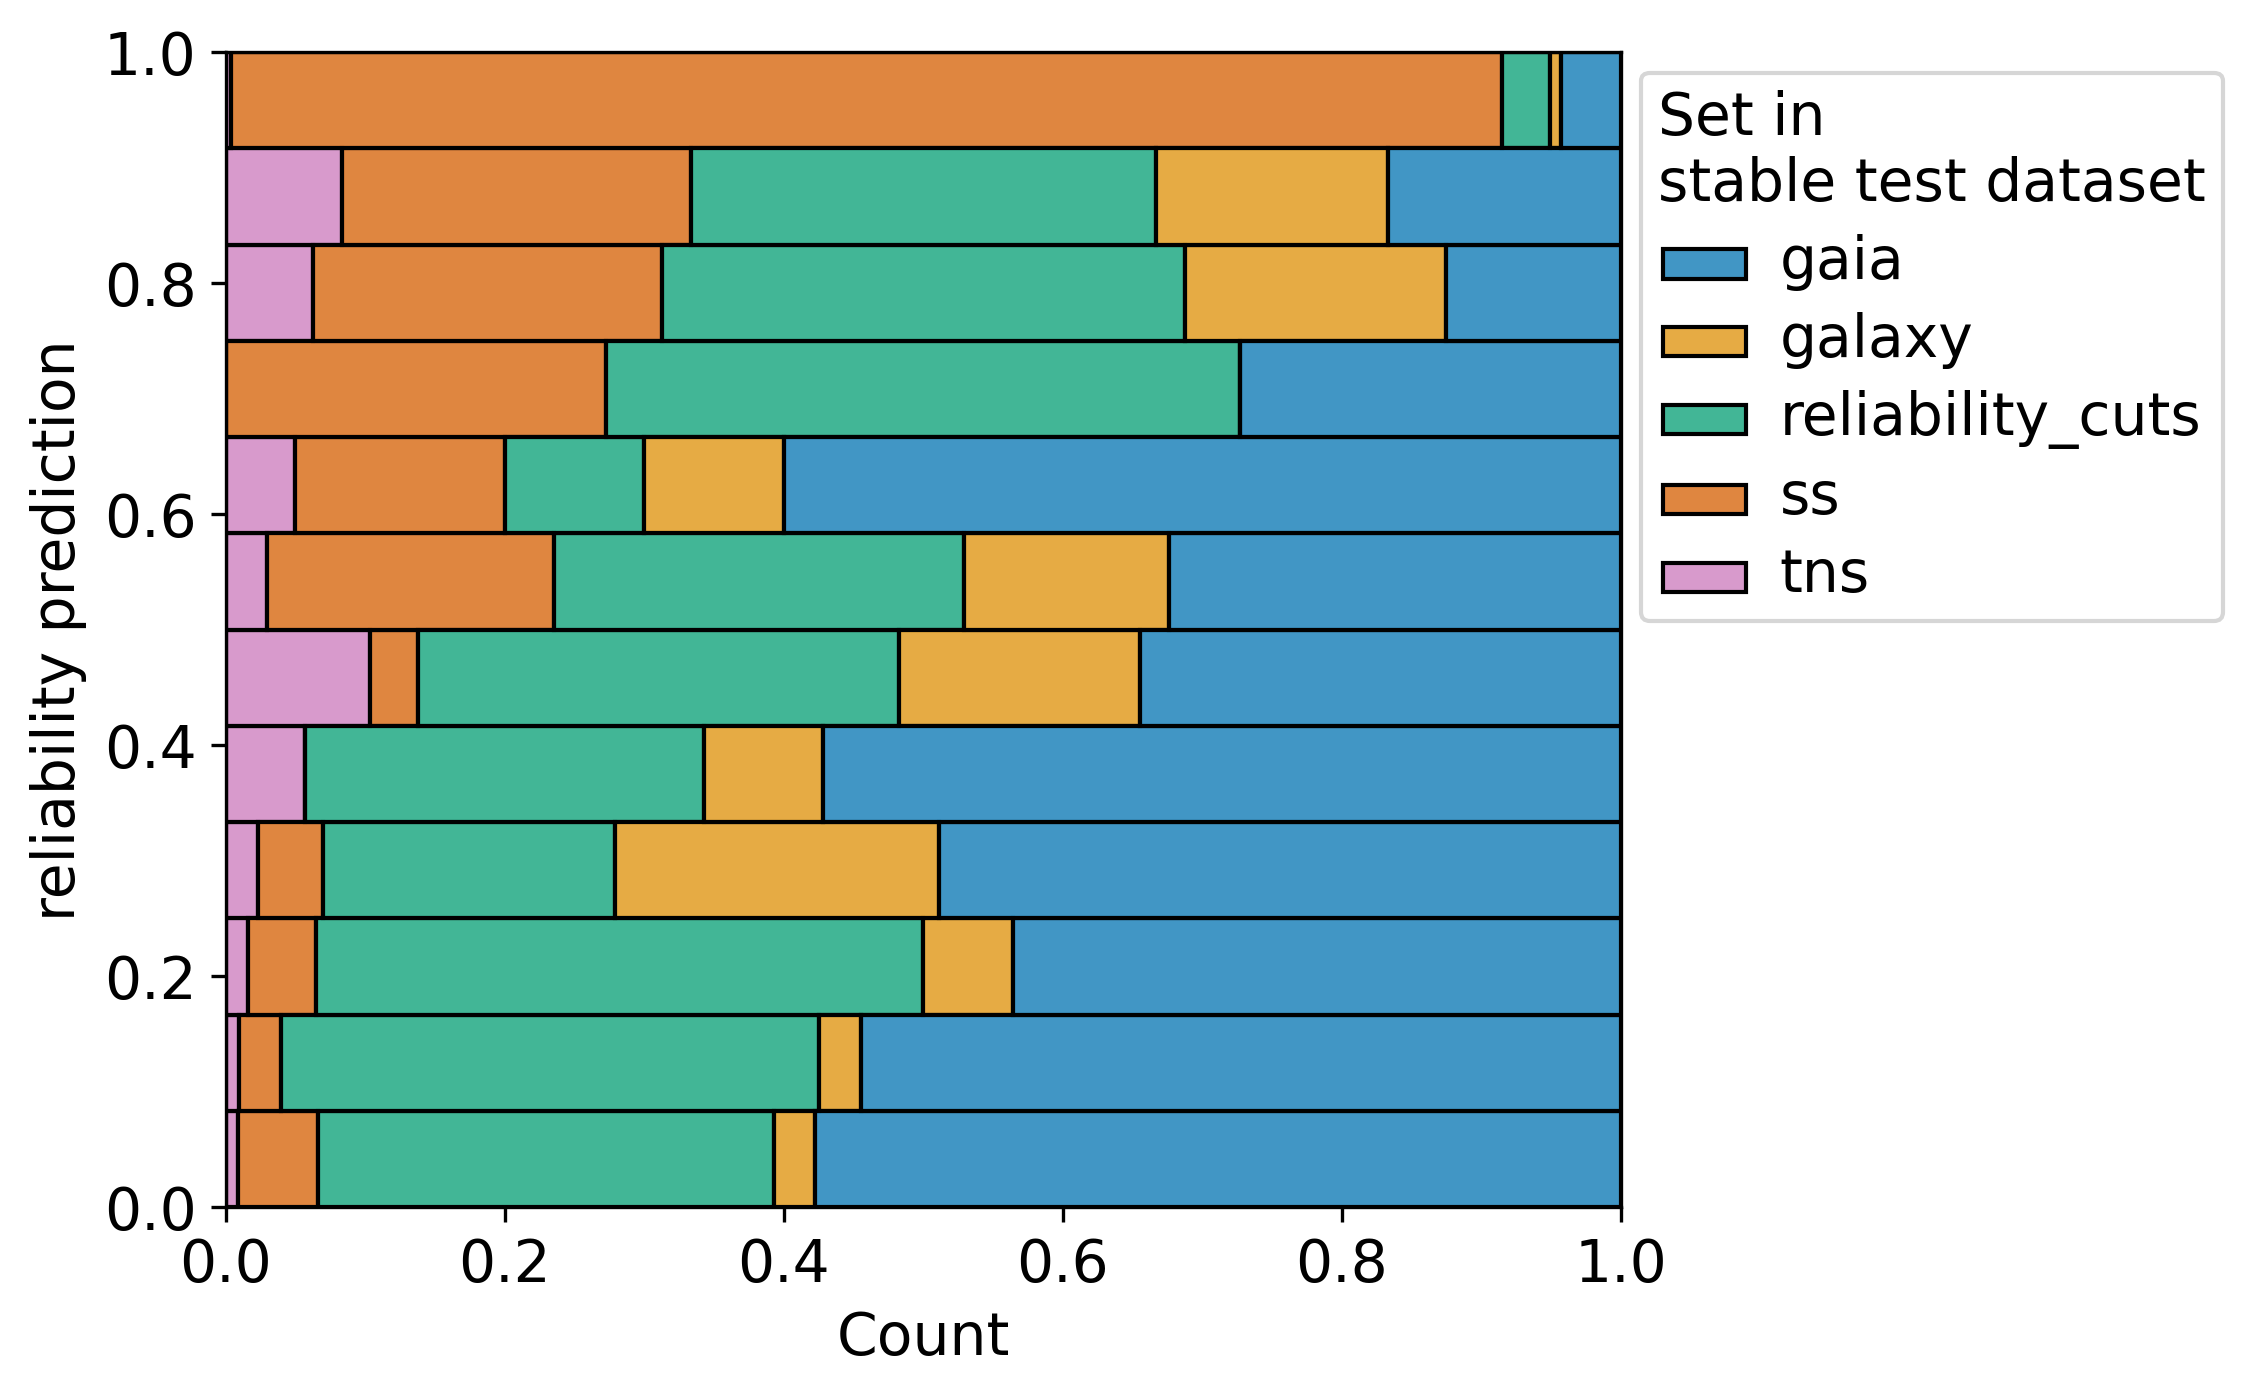
\includegraphics[width=0.45\linewidth]{figures/predictions_stabletest_byset.png}
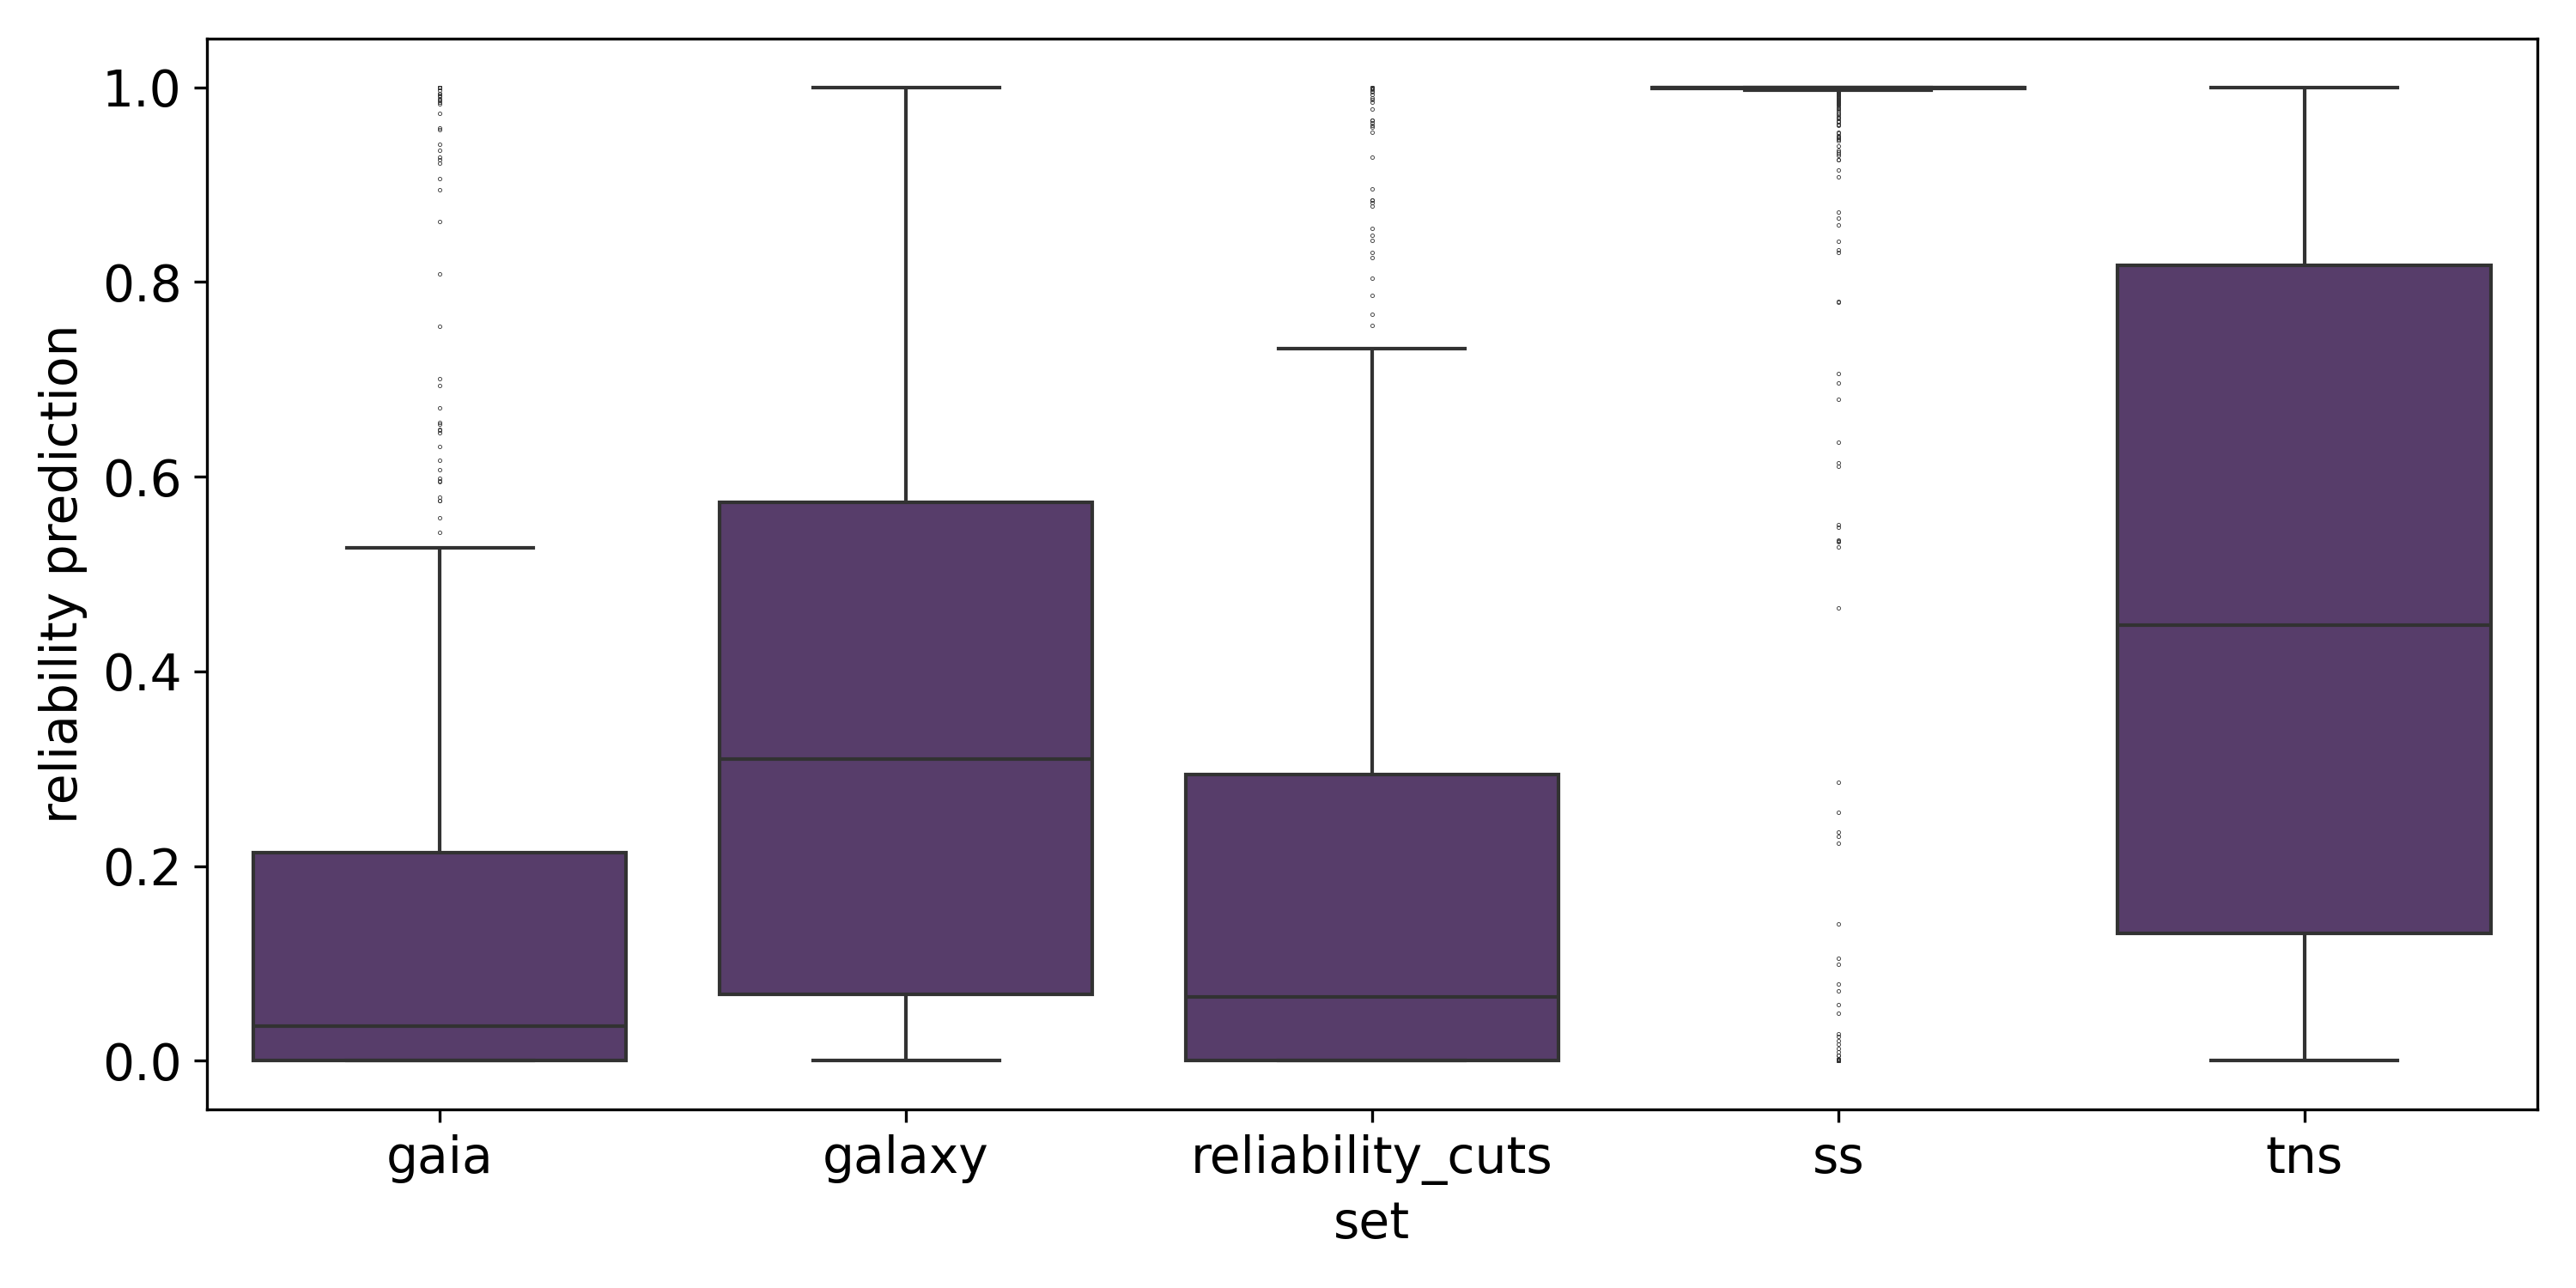
\includegraphics[width=0.48\linewidth]{figures/predictions_stabltest_byset_boxplot.png}
    \caption{Reliability score on test data without fake injections. On the left, the fraction of labels by score range. The majority of high scores come from matches with Solar System objects (see \autoref{sec:data}) while all other sets contribute to all score ranges. On the right, while the distribution of Solar System objects is highly compressed near $\rel=1$ the Gaia cross-matches and  high \V1 score LSSTComCam detections have characteristically low scores.}
    \label{fig:distribution_rel_score}
\end{figure}


\begin{figure}[htb!]
    \centering
    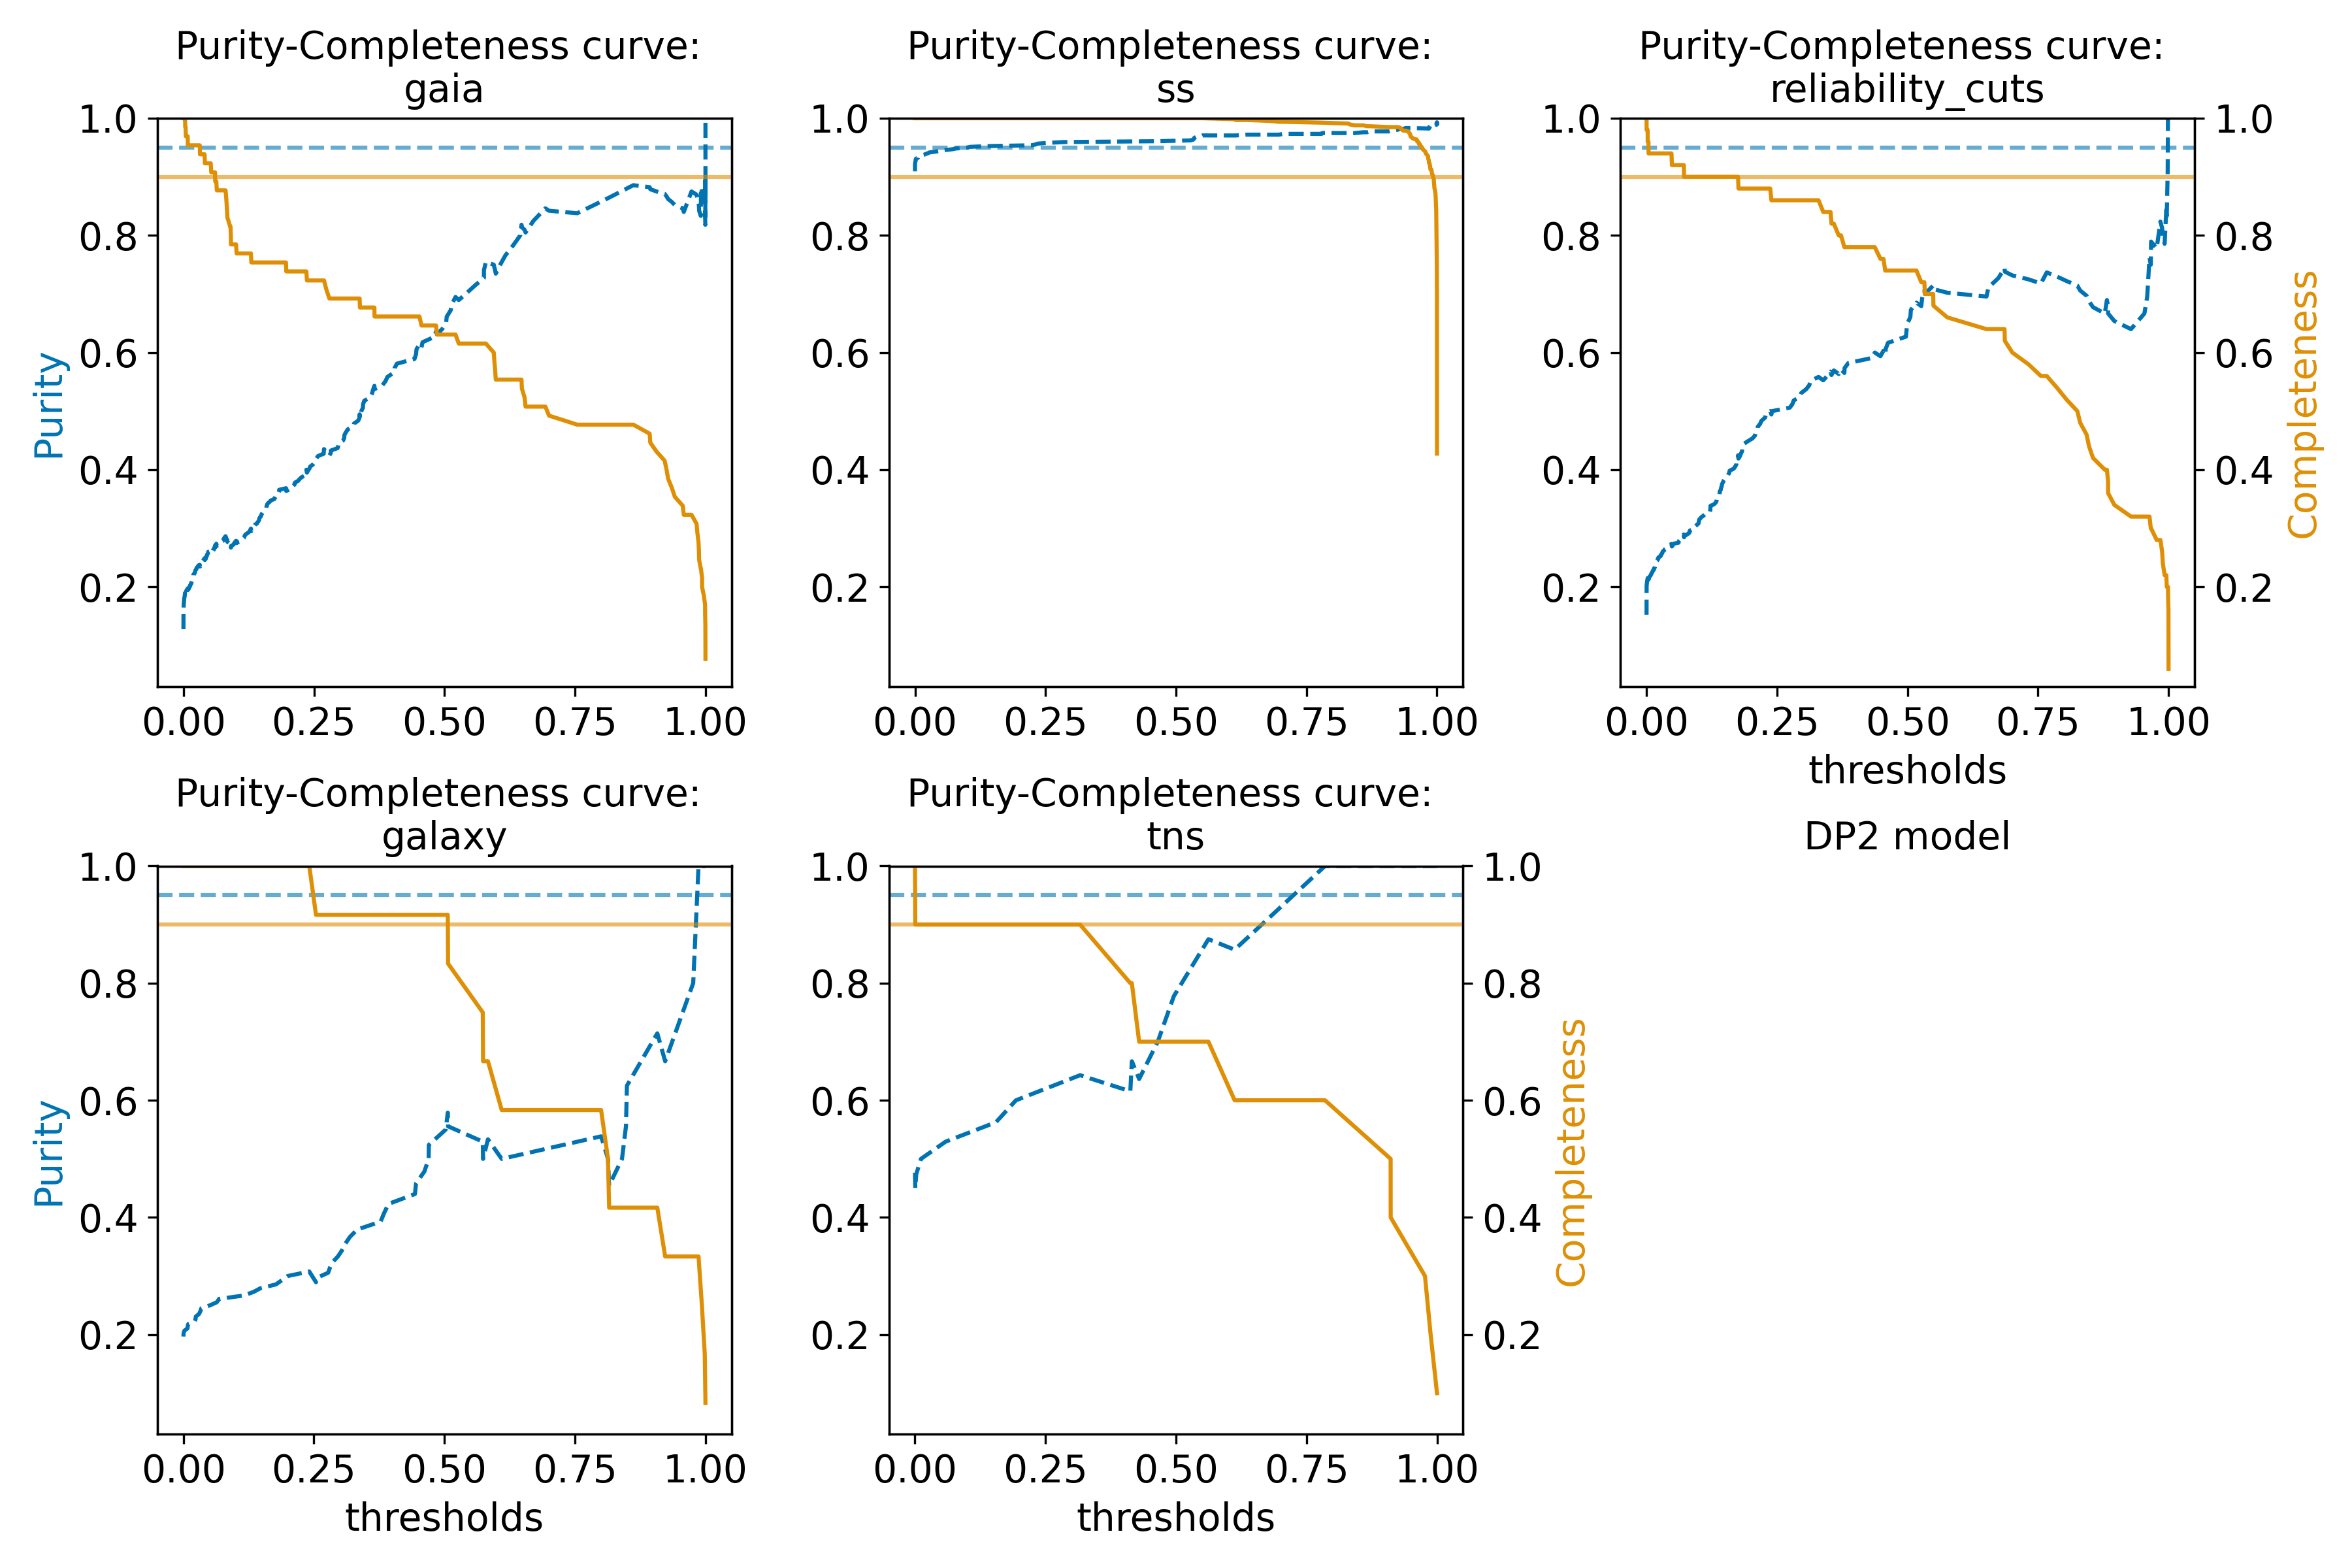
\includegraphics[width=1\linewidth]{figures/stable_byset_dp2_report_new_model.png}
    \caption{Purity and completeness per data origin for test data without fake injection (Zooniverse labels).}
    \label{fig:dp2_performance_byset}
\end{figure}









% \subsection{Future model}
% The construction of the ground truth labels for fine-tuning the model relied on the Zooniverse analysis obtained by considering the training data set of both the Oxford team and the Rubin-ML-Reliability team (see \autoref{tab:total_data_zoo_analysis}). Additionally, we include fakes from more recent injection runs.
% \section{Known Issues}
% \subsection{DP1 model}
% \subsection{DP2 model}




\appendix

\section{Acknowledgements}

This material is based upon work supported in part by the National Science Foundation through Cooperative Agreements AST-1258333 and AST-2241526 and Cooperative Support Agreements AST-1202910 and AST-2211468 managed by the Association of Universities for Research in Astronomy (AURA), and the Department of Energy under Contract No.\ DE-AC02-76SF00515 with the SLAC National Accelerator Laboratory managed by Stanford University.
Additional Rubin Observatory funding comes from private donations, grants to universities, and in-kind support from LSST-DA Institutional Members.

% Include all the relevant bib files.
% https://lsst-texmf.lsst.io/lsstdoc.html#bibliographies
\section{References} \label{sec:bib}
\renewcommand{\refname}{} % Suppress default Bibliography section
\bibliography{local,lsst,lsst-dm,refs_ads,refs,books}

% Make sure lsst-texmf/bin/generateAcronyms.py is in your path
\section{Acronyms} \label{sec:acronyms}
\input{acronyms.tex}
% If you want glossary uncomment below -- comment out the two lines above
%\printglossaries





\end{document}
